\documentclass[12pt]{report}
\usepackage{times}
\usepackage{amsmath}
\usepackage{graphicx}
\usepackage{url}
\usepackage{calc}
\usepackage{subfigure}
\newcommand{\sigline}[1]{\makebox[\widthof{#1~}]{.\dotfill}\\#1}
\usepackage {geometry}
\usepackage{hyperref}
\geometry {
    a4paper, 
    left = 1.25in,
    right= 1 in,
    bottom = 1 in,
    top = 1in,
}
\title{News Text Classification And Comparing Two Different Feature Extraction Techniques}

\author{Dipesh Neupane, Nirmal Gelal, Badri Thapa}
\begin{document}


\pagenumbering{gobble}
    \begin{center}
        
        \begin{figure}
            \centering
            
\includegraphics[scale=0.3]{tulogo.png}
        \end{figure}
    \vskip 1in
    \begin{Huge}
    \textbf{Tribhuvan University}

    Institute of Science and Technology\\[0.5in]
    \end{Huge}
    

    
    
    \begin{Large}
    A Project Report on
    
    \textbf{News Classification: Comparing PLSA and LSA as Feature Extraction Techniques}\\[0.5in]
    \end{Large}
    \emph{for the partial fulfillment of requirement for the degree of}
    
    
    \begin{large}Bachelor of Science in Computer Science and Information Technology

    \textbf{(BSc.CSIT)}\\[0.5in]
    \end{large}
    
    \begin{large}
        \underline{\emph{SUBMITTED BY:}}

        \textbf{Badri Thapa}

        \textbf{Dipesh Neupane}
        
        \textbf{Nirmal Gelal}\\[1.2cm]
    \end{large}
    
    \begin{large}
    \underline{\emph{SUBMITTED TO:}}\\[0.13cm]

    \textbf{Patan Multiple Campus}
    \end{large}

    \begin{large}
    Department of CSIT


    
    \end{large}
    Patandhoka, Lalitpur\\[1cm]
    \textbf{October 7\textsuperscript{th} 2021}
    \end{center}
    \newpage
    \pagenumbering{roman}
    \begin{center}
    \textbf{SUPERVISOR'S RECOMMENDATION}
    \end{center}
    \paragraph{}
        I hereby recommend thta this project prepared under my supervision by Badri Thapa [1508/074], Dipesh Neupane [15016/074] and Nirmal Gelal [15032/074]
        entitled "News Classification and Comparing PLSA and LSA as Feature Extraction Techniques" in partial fulfillment of this requirement for the degree of \textbf{Bachelor in Science in Computer Science and Information Technology (BSc. CSIT)}
        be processed for evaluation. 
        \vspace{3in}

        \begin{center}
        %    \noindent%
           \sigline{Bikash Balami} 
           
           Supervisor
        \end{center}


    \newpage

    \begin{center}
        \textbf{LETTER OF APPROVAL}

        

    \end{center}
\paragraph{}
This is to certify that this project prepared by Badri Thapa, Dipesh Neupane and Nirmal Gelal entitled "News Classification: Comparing PLSA and LSA as Feature Extraction Techniques"
        is in partilal fulfillment of the requirement for \textbf{Bachelor in Science in Computer Science and Information Technology (BSc. CSIT)} has been well studied. In our opinion, it is satisfactory in the scope and quality for the required degree.
        



    \newpage

    \begin{center}
        \textbf{ACKNOWLEDGEMENT}


    \end{center}
    \paragraph{}
        We would like to thank our supervisor Mr. Bikash Balami for his feedback and guidance during the course of this project.
        His contribution in simulating suggestions and encouragement helped us to coordinate our project.

        In addition, we would like to thank the management of Patan Multiple Campus for providing all the necessary guidelines and reference books for the development of 
        our project. 

        We are thankful to the Department of Statistics and Computer Science, Patan Multiple Campus for providing with this opportunity of undertaking a project work and 
        proceeding with it.

    





    \newpage

 \begin{center}
        \textbf{ABSTRACT}
        

    \end{center}
    \paragraph{}
        Classification has been an important challenge in the ongoing research in the context of Nepali Texts.
        With the abundancy of the Nepali language texts in recent years - mainly due to the availability of internet and 
        popularity of it, there has been a number of literatures been written to tackle it. 

        Although, in languages like English this is not a new domain of research, it is in early-stages in Nepali Language. And, with a large 
        number of unstructured texts available in the internet, classifications tasks are difficult to achieve. A main problem to achieve a proper 
        classification is to convert the unstructured documents into well-structured relevant format. 

        The purpose of this project is to find a automatic feature extraction techinque that can represent the document well enough so that the classificaiton can be
        done easily and with a relatively small data sample. Latent Semantic Analysis and Probabilistic Latent Semantic Analysis are two of the old-school 
        feature extractor which are compared in this project and want to gain insights on which can be an optimum techinque for extracting features from the Nepali texts.
        
        


    \newpage


    \begin{center}
        \textbf{
            List of Abbreviations
        }

       



    \end{center}
    \textbf{LSA} ................... Latent Semantic Analysis


    \textbf{SVD} ................... Singular Value Decomposition

    \textbf{TF-IDF} ................ Term-frequency Inverse-Document Frequency
    
    
    \textbf{PLSA} .................. Probabilistic Latent Semantic Analysis


    \textbf{SVM} ................... Support Vector Machines


    \textbf{k-NN} .................. K Nearest Neighbors


    \textbf{SLSA} .................. Supplemented Latent Semantic Analysis
    

    \newpage

    \tableofcontents
    \newpage
    \pagenumbering{arabic}
    \chapter{Introduction}
    
    \section{Introduction}
    \paragraph{}
        Human beings have used text as a form of communication of their thoughts and knowledge from ancient times. All over the world, most civilizations have developed their some form of textual symbols 
        (alphabets), and  their own grammers.
        And Nepal is no exception to that. Nepali language evolved from Sanskrit, and the 36 consonants, 12 vowels and 10 numerals also known as Devanagari found in Nepali writings is also found 
        in the Sanskrit language. 
        These characters have their own variants, along with some special characters. All in all, Nepali language is a rich and complicated language with interesting grammer and symbols to write it with.
        
        Nepali writings has had a significant rise in internet in recent times. With that, there is need of a automatic processing of such writings.          
        So, in this project, the news articles in Nepali language will be classified into different topics (categories) and also identify keywords associated with the topic.
        It is also a problem of document classification which is the task of assigning a document to one or more categories. It is a supervised learning task. 

        The idea of document classification problem is to assign the document to one or more class. The class maybe the abstract topic a collection of document represents. The topic may be philosophical, or, scientifically represetative
        of the collection of the documents. There are many techinques for autoamtic classification of documents, such as, Expectation Maximization, Naive Bayes Classifier, TF-IDF, LSA, Support Vector Machines,
        neural networks, etc, and are used in spam filtering, email routing, language identification\cite{wikipedia2021}. 
        

        
        
        



        

        
    \section{Problem Statement}
        Document Classification and topic modeling is a classic problem in machine learning. It has had massive research and there have been many procedures described and
        constructed to discover solutions to such problems. with a significant rise in Nepali text/articles in the internet, a lot of problems may come 
        while sorting the articles and texts. And Latent Semantic Analysis and Probabilistic Latent Semantic Analysis is one of those techniques that attempts 
        to cluster the documents in an unsupervised way. And it can also be a powerful feature extraction techinque which can then be used for document classification using a 
        supervised learning method. Although, they are quite similar they incorporate different ideas and have their own advantages. So, by applying these techniques for document classification, 
        the advantages and disadvantages of these techniques can be realized. 
    
    \section{Objectives}
        The aim of this project is find out if LSA or PLSA can be good tool for extracting features the Nepali news articles topic-wise.

    
    \section{Scope and Limitations}
        
        \subsection{Scope}
        The project was developed to find a computationally fast way to automatically extract features from the text corpus. 
        The features must be representative of the text corpus and should enable for better precision for classification tasks. 
        Also, the project should establish a proper preprocessing steps for better feature extraction.

        \subsection{Limitations}
        The project contains some limitation such as a single document cannot be used for the feature extraction using these techniques.
        Stemming of the Nepali texts is not reliable. Due to typos, many words with significance are lost. Some descrepancies in Nepali Unicode values 
        causes some punctuations hard to remove. Large number of documents is very hard to parse through and process due to limited computational devices.


    \section{Development Methodology}

        Extracting features from the text corpus so that the computer can understand and learn from it consists of well-described
        series of steps which are:
        

        
        \subsubsection{Dataset Collection}
            A scrapper was built and used to collect the news articles from various websites like Ekantipur, Ratopati, Setopati, ReportersNepal and OnlineKhabar.
            A total of 12 categories were scrapped off these websites namely: Business, Education, Entertainment, Health, Interview, 
            Literature, National, Opinion, Sports, Technology, Tourism, and World. Although, only 10 categories were only used and Opinion and Interview were discarded.


        \subsubsection{Preprocessing}
            To preprocess the text means bringing the text into a form that is predictable and analyzable for any task. The preprocessing of the text in our case
            makes it ready to be used in training and testing of the machine learning model. Preprocessing is mainly done to reduce the noise the text that 
            helps to imporve the performance of the classifier and speed up the clsssifcation process, thus aiding in real time news classification. The text preprocessing may 
            include: lowercasing, stemming, tokenization, special symbols and number removal(noise removal), lemmatization, stopword removal, normalization, and some others. 
            Here, following operations are carried out for preprocessing of the text:
            \begin{description}
                \item[1. Tokenization:]
                     It is one of the common taks in Natural Language Processing. It is a way of separating a peice of text into smaller units called tokens. 
                    It can either be words, characters, or subwords. Here, a word is taken as a single token. It is mostly separated by a white spaces, or using some special symbol.
                \item[2. Special symbol and number removal:] Special symbols like $~{!, |, }~$ \textbackslash, 
                $~{ \div, \%, \$, -,}~$ \newline $~{(, ), /, <, >, =, +,}~$  \textasciicircum, etc. and numbers, those which do not have much importance in classification, are removed.

                \item [3. Stop word removal:] Stop words are such words which are too frequent among the documents in the collection. Such words 
                    which occur too frequently are useless for purposes of retrieval. They are normally filtered out. Articles, prepositions, and conjunctions
                    are natural candidates for a list of stopwords.
                \item [4. Stemming:] It is the process to reduce a word into its stem. A stem is the portion of a word which is left after the removal 
                    of its affixes (i.e. prefixes and suffixes). The stemmer used is a developed module found in \url{https://pypi.org/project/nepali-stemmer/}.
                
            \end{description}
            \subsection{Exploring the preprocessed Data}
            After the preprocessing the data was then analyzed. It was seen that there were a lot of typos in the texts. 
            \begin{figure}[!htb]
                \begin{minipage}{0.48\textwidth}
                  \centering
                  
\includegraphics[width=.7\linewidth]{typo11.png}
                  \caption{a single word which should be three different words}\label{Fig:typo1}
                \end{minipage}\hfill
                \begin{minipage}{0.48\textwidth}
                  \centering
                  
\includegraphics[width=.7\linewidth]{typo22.png}
                  \caption{a single word which should be two different words}\label{Fig:typo2}
                \end{minipage}
             \end{figure}

             \begin{figure}[h]
                 \centering
                 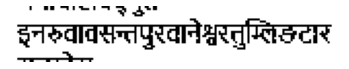
\includegraphics[width=.7\linewidth]{typo33.png}
                 \caption{a single which should be many different words}\label{Fig:typo3}
             \end{figure}

            Another kind of typos that was encountered - same word is written in different ways. This main happened 
            because of people writing the foreign words in Nepali. So, the spelling for the same word was different.
            
            \begin{figure}[h]
                \centering
                \subfigure[]{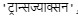
\includegraphics[width=0.24\textwidth]{typo4.jpg}} 
                \subfigure[]{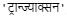
\includegraphics[width=0.24\textwidth]{typo5.jpg}}
                \subfigure[]{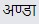
\includegraphics[width=0.20\textwidth]{typo6.jpg}}
                \subfigure[]{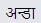
\includegraphics[width=0.20\textwidth]{typo7.jpg}}



                \caption{(a) and (b) is the same word but has different spellings making them distinct and same with (c) and (d)}
             \end{figure}

            This led to counting of the distinct words in the corpus. The unique word count was too high and all the words which had the 
            word count of 1 in the corpus was deleted. Then, we randomly deleted half the corpus since the document-term matrix would not 
            fit in the memory of eight gigabytes.


            \subsubsection{Data Preparation}
        
            After preprocessing the data was divided into several sets of different sizes for more comparative studies. There were four sets of 1600, 1200, 1000 and 500 documents.
            Each sets of documents were fed into the feature extraction pipeline and then into the machine learning algorithms for comparison.
            
        
        \subsubsection{Feature Extraction}
        After the initial text is cleaned and normalized, it is required to extract the features to be used for modeling.
        These words that are within our documents are assigned weights before modeling them.
        


        In order to cluster and then classify the document, the document must be represented into a mathematical form. There are some ways to represent documents and the three classic models are, namely, 
        Boolean, the vector, and the probabilistic models\cite{baeza1999modern}. In this project, the vector space model is used\cite{salton1975vector} to convert the document into a mathematical form. These vectors are formed using the terms \emph{t} occurring in the documents 
        as the elements of the document vector. The simplistic approach to represent the document and the ability to do partial matching and calculating the degree
        of similarity between documents makes it a very optimal choice. 
        \begin{figure}[h]
            \centering
            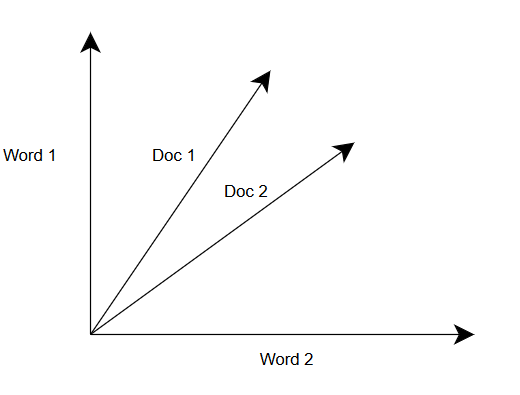
\includegraphics[scale=0.7]{vectorrep.png}
            \caption{\textbf{The vector representation of document.}}
        \end{figure}
        \paragraph{}Formally, if \emph{t} different terms are present in the document and each document is represented by a t-dimensional vector, then 
        
        \begin{center}
            
          $~{D_i = \{d_{i1}, d_{i2},....,d_{it}\} ,}~$ 
        
        \end{center} 
        
        $~{d_{ij}}~$ representing the "weight" of the jth term\cite{salton1975vector}.

        And, the similarity between the two documents can be then calculated as:
       
            \begin{equation}
                  sim(d_j, q) =  \frac{  \vec{d_j} \cdot \vec{q}  } {|\vec{d_j}|  \times |\vec{q}|  }   
                = \frac{\sum_{i=1}^{t}w_{i,j}\times w_{i,q}} {\sqrt{\sum_{i=1}^{t}w_{i,q}^2} \times \sqrt{\sum_{i=1}^{t}w_{i,j}^2}}
            \end{equation}
            where, \textit{$~{d_j}~$} and \emph{q} are the two documents as t-dimensional vectors, $~{w_{i,j}}~$ and $~{w_{i,q}}~$ are the weights of the terms, and the calculated value is known 
            as the \emph{cosine of the angle} between these vectors\cite{baeza1999modern}. And the $~{|\vec{d_j}|}~$ and $~{|\vec{q}|}~$ are the norms of the documents.
        
            The easiest way to represent individual words is the numerical representation as it's easy for the computer to process numbers. Some of 
        the extractions techniques are Bag of words, TF-IDF, One-hot Encoding, and word embeddings. 
        Here TF-IDF\cite{schutze2008introduction} is used as the feature extraction technique and the document is transformed into a vector form.
        To represent Nepali news in vector form, the TF-IDF weighting value for each word in the text is taken as a high dimensional
        value in a vector. It is calculated as,    
        \begin{equation} W_{t, d, D} = tf_{t, d} * idf_{t, D} \end{equation}  
         where,\newline
        $~{tf_{t, d} = \frac{f_{t,d}}{max\{f_{t', d} : t' \in d\}}}~$ \newline
        $~{idf_{t, D} = \log \frac{N}{1+  | {d \in D: t \in d}  |}}~$ \newline
            and,\newline
        $~{tf}~$ = term frequency\newline
        $~{idf}~$ = Inverse document frequency\newline
        $~{f_{t,d}}~$ = Number of term t in document $~{d}~$\newline
        $~{max\{f_{t', d} : t' \in d\} }~$ = max occurring term $~{t'}~$ in document $~{d}~$.\newline
        N = Total number of document in the corpus $~{D}~$.\newline
        $~{|{d \in D: t \in d}|}~$ = Number of documents where the term $~{t}~$ appears. \newline

        All this can be possible to be done only after the documents are subjected to the technique of Latent Semantic Analysis (LSA)\cite{deerwester1990indexing} 
        which reduces the
        original term-document matrix \textbf{D} into a filtered term-document matrix. Here, the term-documents matrix can be the collection of vector of the documents. 
        The vector may be a row or a column of the matrix. 
        This method uses a mathematical technique called \emph{Singular Value Decomposition} to identify patterns in the relationships between the terms and 
        concepts contained in the collection of texts. It represents the meaning of a word as a kind of average of the meaning of all the passages in which it appears, 
        and the meaning of a passage as a kind of average of the meaning of all the words it contains\cite{landauer1998introduction}. 
        This method takes a large matrix (combination of vectors) of term-document data and constructs a "semantic" space wherein terms and documents that are closely associated 
        are placed near one another. 
        
        The SVD decomposes the original matrix into three matices: a document-topic matrix, and Singular matrix, and a term-topic matrix. 
        The SVD for a matrix(rectangular) \textbf{D} can be given as:
        \begin{equation}\label{eq1}
            \mathbf{D} = \mathbf{U} \Sigma  \mathbf{V^T}
        \end{equation}
        
        where \textbf{U} with ${t \times r}$ is the terms-topic matrix, ${\Sigma}$ with ${r \times r}$size is the array of Singular values and 
        the ${\mathbf{V^T}}$ with ${r \times d}$ is the document-terms matrix. 
        The singular values show the relative importance of our topic. \textbf{U} and ${\mathbf{V^T}}$ are orthonormal matrices and the ${\Sigma}$ is a diagonal matrix which has values 
        in descending order in the diagonal.
        \begin{figure}
            \centering
            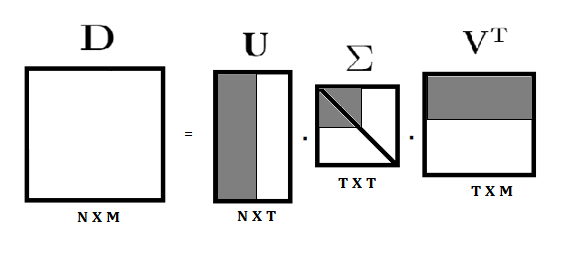
\includegraphics[scale=0.7]{lsa.png}
            \caption{\textbf{The figure shows how the document-term matrix is decomposed into its subsequent three low rank matrices. The shaded portion shows how much 
            values can be truncated and approximate the original matrix. Note: shaded portion is taken to approximate the original matrix \textbf{D}.}}
        \end{figure}
        Intuitively, in linear algebra, the three matrices rotate (\textbf{U} and ${\mathbf{V^T}}$) and scale (${\Sigma}$) the space and is the same as doing 
        the transformation with \textbf{D}. 
        The process of decomposing into the three matrices will not be discussed. Although, the essence of SVD, that is, the dimensionality reduction, is to be discussed. 
        Since the singular values describe how each latent concept explains the variance in our data, the number of values (concepts) has to be chosen so that the original
        matrix can be approximated with minimal error. This will be mapped into a lower-dimensional space. They will be a lower-dimensional approximation of the higher-dimensional space. 
        The reason for this to do is that, the original matrix may be too large, sparse and noisy. And it assumes that after rank lowering that some dimensions are combined and
        depend on more than one term. This will lead to merge the dimensions associated with terms that have similar meanings. And conversely, the terms that have opposite or no 
        association with them will either cancel out, or, at least, be smaller than that with similar meanings.
        This process of selecting the \emph{k} largest singular values, and their corresponding singular vectors from \textbf{U} and ${\mathbf{V^T}}$ is known as the dimensionality reduction step. 
        Here, the number of singular values chosen will be directly related to the number of concepts to be separated and defined.
        This finaly step will lead to many things. First, the comparison between the document will occur in the low-dimensional space. The terms related with each other will be found out. 
        The importance of the term for the concept can be seen as well. Hidden word association can be analyzed as well.   
        Overall, the following steps can be done for low rank approximation using SVD:\\
        1. Given \textbf{D}, construct its SVD in the form as ${\mathbf{D} = \mathbf{U} \Sigma  \mathbf{V^T}}$.\\
        2. Derive from ${\Sigma}$ the matrix ${\Sigma_k}$ formed by taking the first \emph{k} singular values and replacing others with 0.\\
        3. Compute and output ${\mathbf{D_k} = \mathbf{U} \Sigma_k  \mathbf{V^T}}$ as the rank-k approximation to \textbf{D}.\cite{cambridge2009online}
        
        Although, LSA is a relatively simple technique, it sure has some downsides. Such as the relative importance of a word cannot be found out from the decomposed matrix. 
        It is also hard to infer what the numbers in LSA is telling us and can be negative values. With regard to that, another technique for topic modeling and document classification
        was introduced, called as probabilistic Latent Semantic Analysis. As the name suggests, it models co-occurrence information under a probabilistic framework in order to 
        discover the underlying semantic structure of the data. It was developed in 1999 by Thomas Hofmann\cite{hofmann2013probabilistic}. Initially, it was used for text-based
        application, however it has slipped onto other fields: such as computer vision or audio processing. 
        Probabilistic latent semantic analysis is an expectation maximization-based mixture modeling algorithm\cite{aggarwal2015data}. There exists a generative process \cite{aggarwal2015data}
        inherently for dimensional reduction and builds the document-term matrix as follows (with $~{Z_m}~$ as a topic, $~{d_i}~$ as document and $~{w_j}~$ as a word token ):
        \begin{itemize}
            \item Select a document $~{d_i}~$ with probability $~{P(d_i)}~$.
            \item Generate the probabilities $~{P(Z_m|d_i)}~$ for a latent class (topic) and $~{P(w_j | Z_m)}~$ for a word and put it in the relevant indices of the document-word pair $~{(d_i, w_j)}~$. Here, 
            document and word is assumed to be \emph{conditionally independent}.

        \end{itemize}
        \begin{figure}[h]
            \centering
            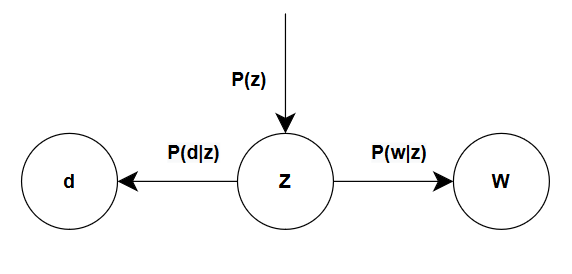
\includegraphics[scale=0.5]{graphrep.png}
            \caption{\textbf{The figures shows how the latent topic \emph{z} can make a conditional independence between the 
            document \emph{d} and the words occurring in the document \emph{w}. It is the graphical representation of the aspect model.} }
        \end{figure}
        The conditional independence between the words and the documents is an important assumption in PLSA given the latent aspect 
        in our case, the topic. Which actually means:
        \begin{equation}P(d, w) = P(d) P(w|d), P(w|d) = \sum_{z \in Z}^{} P(w|z) P(z|d) \end{equation}
        It means that the joint probability between the documents and words pair can be expressed in the following way:
        \begin{equation}\label{eq4}
            P(d, w) = P(d) \sum_{z \in Z} P(z|d) P(w|z) = \sum_{z \in Z} P(z) P(d|z) P(w|z) 
        \end{equation}
        The conditional independence assumption makes it possible for the derivation of \emph{EM algorithm}.
        Initially, the EM algorithm starts by initializing $~{P(Z_m), P(d_i|Z_m),}~$ and $~{P(w_j|Z_m)}~$ to 1/k, 1/n and 1/d, respectively.
        Here, k, n, and d denote the number of clusters (topics), number of documents, and number of words, respectively. 
        \begin{enumerate}
            \item \textbf{E-step} The posterior probability is calculated using the equation:
                    \begin{equation}
                        P(z|d, w) = \frac{P(z) P(d|z) P(w|z)}{\sum_{z' \in Z} P(z') P(d|z') P(w|z')}
                    \end{equation}
            \item \textbf{M-step} The $~{P(Z_m), P(d_i|Z_m)}~$ and $~{P(w_j|Z_m)}~$ is calculated by:
                    \begin{equation}
                        P(w|z) \propto \sum_{d \in D} n(d, w) P(z|d, w),
                    \end{equation}
                    \begin{equation}
                        P(d|z) \propto \sum_{w \in W} n(d, w) P(z|d, w),
                    \end{equation}
                    \begin{equation}
                        P(z) \propto \sum_{d \in D} \sum_{w \in W} n(d, w) P(z|d, w).
                    \end{equation}
        \end{enumerate}
        These two steps are iteratively repeated until convergence. The convergence is done using the maximization of the log likelihood 
        function:
        
         \begin{equation}
             \mathcal{L} = \sum_{d \in D} \sum_{w \in W} n(d, w)  \log P(w, d)   
         \end{equation}
        Although the original paper \cite{hofmann2013probabilistic} used a method called 
        \emph{Tempered Expectation Maximization} in order to avoid overfitting.
        
        Also, the PLSA can be seen as a matrix factorization as well. The factorization of the co-occurrence of the 
        document matrix can easily be seen using equation \ref{eq4}. It can also be seen as:
        \begin{equation}\label{eq10}
            P = U \cdot \Sigma \cdot V
        \end{equation}
        \begin{figure}[h]
            \centering
            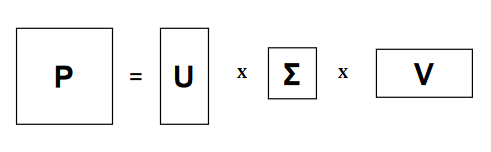
\includegraphics[scale=0.8]{plsa.png}
            \caption{\textbf{The matrices can be representation of the probabilistic latent semantic analysis.}}
        \end{figure}
        where each matrix means:
        \begin{itemize}
            \item U contains the document probabilities $~{P(d|z)}~$.
            \item $~{\Sigma}~$ has diagonal elements with of the prior probabilities of the 
            topics $~{P(z)}~$.
            \item V contains the word probability $~{P(w|z)}~$.
            \item P means the $~{P(w,d)}~$.  
        \end{itemize}
        
        The main advantage here of this representation over LSA is that the entries are normalized and 
        have no negative values. And the value represents the importance of each entry for given topic.
        
               
        
        
        The TF-IDF can only be used for LSA. Then, Singular Value Decomposition is applied. 
        While for pLSA, Bag of Words is used for the creating a document-matrix form and estimate the $~{P(w, d), P(d|z), P(z) and P(w|z)}~$. 

        \subsubsection{Feature Extraction Details}

            In LSA, the number of topics had to be hand-picked and 10, 50, 100 were chosen for dimensional reduction. 
            In pLSA, the algorithm was much more computationally expensive and only 10 was chosen for the number of topics.


        
        \subsubsection{Machine Learning}
        After the feature extraction has been done for both pLSA and LSA, supervised machine learning algorithms like Logistic Regression, Support Vector Machines and Random Forest Classifier are trained
        on the document-term matrix. Each set was divided into a 90-10 training-validation split. The validation for each was used to test the algorithm's 
        performance on each set.
        
        \paragraph{Logistic Regression}
        
        is a linear model for classification and is also known as logit regression, maximum-entropy 
        classification or the log-linear classifier. 
        In this model, the probabilisties describing the possible outcomes of a single trial are modeled using a logistic function.

        A logistic function is a common S-shaped curve (sigmoid curve) with equation 
        \begin{equation}
            f(x) = \frac{1}{1+ e^{-x}}
        \end{equation}

        \paragraph{Support Vector Machines}
        
        
        are a set of supervised learning methods used for classification, regression and outliers detections.
        A support vector machine constructs a hyper-plane or set of hyper-planes in a high or infinite dimensional space, which can be used for classification,
        regression or other tasks. A good separation is achieved by the hyper-plane that has the largest distance to the nearest training datat points of any class of the classifier.

        \paragraph{Random Forest Classifier}
        
        is one of the ensemble methods that combines the predictions of several base estimators -- decision trees in this case --built with a given learning algorithm 
        in order to improve generalizability / robustness over a single estimator.  


        \section{Project Roadmap}
        Chapter 2 details the words that has been carried out previously in the field of classification of texts in Nepali and other languages. 
        
        Chapter 3 covers the different requirements like functional, non-functional and system requriement of the system.

        Design of the system is discussed in Chapter 4 with different diagrams.

        Implementation methods and system testing data and result are described in Chapter 5.

        The concluding Chapter 6, concludes the chapter explaining what have been done in the project and what further improvements could be done.





    \chapter{Literature Study}
    
            \section{Literature Review}
                \paragraph{}
                    Several notable papers have been written in classification of texts in Nepali and other languages. Only in recent times the classification of Nepali news articles have been done.
                    All have mostly used their own datasets by scrapping the online news portals (in case of Nepali news). They are mostly supervised. The use of PLSA in Nepali language has still not been found.
                    
                    \paragraph{Works related to other language}
                            \cite{pu2006short} used LSA as a data preprocessing method, and then used Independent Component Analysis (ICA) for the classification. They showed that 
                            using ICA and LSA together provides better classification for Chinese short-texts rather than using ICA alone. 
                            
                            \cite{cardoso2003empirical} compared the LSA, SVM, and k-Nearest neighbor variations of the LSA models and showed that SVMs and k-NN LSA performed better 
                            than the other methods that they had compared to. They had evaluated the performance of the models using Mean Reciprocal Rank and argued that it is very well
                            suited evaluation measure for text categorization tasks and the tests were performed on two different datasets (both in English language). They also showed that LSA performs better 
                            when it has many training examples. They also showed that the number of terms in the dataset do not influence the models' performance. 

                            \cite{krishnamurthi2017including} used a modification of the LSA and compared with the traditional LSA. The modified LSA, called
                            SLSA (supplemented latent semantic analysis) added extra information (the label of the document) in the original document matrix 
                            and performed SVD on it. It was shown that this added information had increased the accuracies on classification tasks by 1.14\%, 1.3\% 
                            and 1.63\% for various term weighting schemes (tf, idf, tf-idf). The classification task was done on Hindi texts. 

                            \cite{krishnamurthi2016understanding} also used another modification of LSA by providing supplementary information. They provided 
                            document category and domain information as supplementary information. They showed an improvement of 4.7\% - 6.2\% using this modification which shows that 
                            summary of the text can be additional informaion that can be fed into the model to make it better.

                            \cite{nipu2017machine} used LSA for ambiguity checking in Bengali literature. They showed that the Vector Space Model and LSA gives generally reasonable
                            outcome for Bengali language structure and sentence structure. 

                            \cite{hofmann2013probabilistic} introduced the probabilistic latent semantic analysis and used a Tempered Expectation Maximization algorithm and showed how it was
                            significantly better than the LSA.         
                    \paragraph{Works related to Nepali Language}

                        In Nepali Language, several works have been done, such as, 
                        \cite{sitaula2021vector,shahi2018nepali,kafle2016improving,subba2019nepali,singh2018nepali}. \cite{sitaula2021vector} proposed their own method where they used probability-based
                        word embedding. And they showed that their method was the best classifier among other models. 
                        
                        \cite{shahi2018nepali} used TF-IDF method for feature extraction of Nepali news documents and classified using Naive Bayes, SVM and Neural Networks. 

                        \cite{kafle2016improving} performed a comparative study of various different document representation methods, including LSA, TF-IDF and word2vec. They showed that the accuracy
                        of the TF-IDF with LSI model is far superior than those other two models. 

                        \cite{subba2019nepali} used Bag of Words\cite{salton1983introduction} of the Nepali news articles to train the deep learning network. \cite{singh2018nepali} used TF-IDF for 
                        feature extraction of various Nepali texts and built a model using Logistic Regression, SVM, Multinomial Naive bayes, Bernoulli Naive Bayes, Nearest neighbor and some others as well.

                        In summary, a lot of works done in both Nepali and other languages were found and there were a lot of different methods applied. LSA had been extensively used in 
                        other languages but in Nepali texts, it was a rarity. Works in Nepali used TF-IDF and Bag of Words as a feature extraction and had a wide use of neural networks and other 
                        supervised classification techniques. 



            \chapter{System Analysis}

            \section{Requirement Analysis}
            It defines the scope of the project in the Project Description. It describes the hardware and software components of a system required to develop and use software 
            efficiently.
            The requirements may be functional and non-functional and both are essential to a successful software project. 
            The following Functional and non-functional requirements were identified on the system.

                \paragraph{Functional Requirement}
                The functional requirements defines function of the system where functions are the collective sets of
                input, their behaviors and their output.
                    The application should calssify the atricle into a single topic from a group of different topics based on its contents.
                    \begin{figure}[h]
                        \centering
                        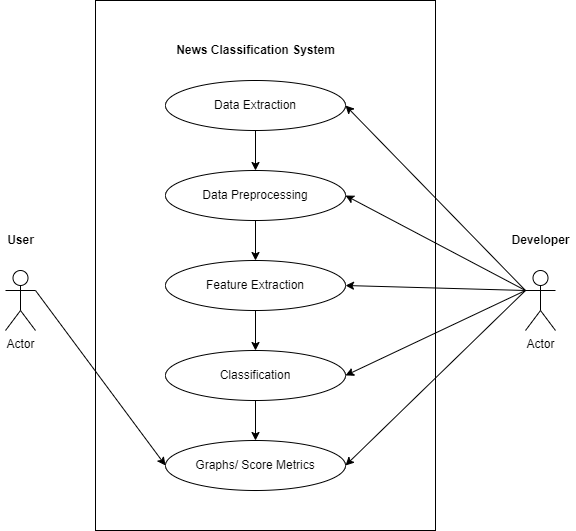
\includegraphics[width=15.29cm, height=14cm]{usecase.png}
                        \caption{\textbf{Use-case diagram of the proposed system.}}
                    \end{figure}
                    \newpage 
                    
                
                \paragraph{Non-functional Requirement}
                Non-functional requirement is a requirement that specifies criteria that can be used to judge the
                operation of a system, rather than specific behaviour.
                    The application should be consistent at classification whenever same article is passed into  the pipeline. 
                    
                    Proper dataset should be built to train and extract features from for the classification. 
            
        \section{Feasibility Study}
            
            \subsection{Technical Feasibility}
            
            Technical analysis is concerned with determining how feasible a system is from a technical
perspective.
                The application would require some degree of technical and coding expertise to run and understand the results.

            \subsection{Economic Feasibility}
            Economical analysis is the study that determines whether a system is economically acceptable or
not.
                The application is economically feasible as there is no extra cost needed to run the program.
            \subsection{Operational Feasiblity}
            It is concerned with the operating capabilities of the system.
                It is concerned with operating capabilities of the system. It will require a decent computer with 8 GigaBytes of RAM and a modern CPU. 

             
        \subsection{Project Timeline}
        Typically Schedule feasibility means estimating how long the system has taken to develop, and if
it can be completed in a given time period using some methods like payback period.
                \begin{figure}[h!]
                    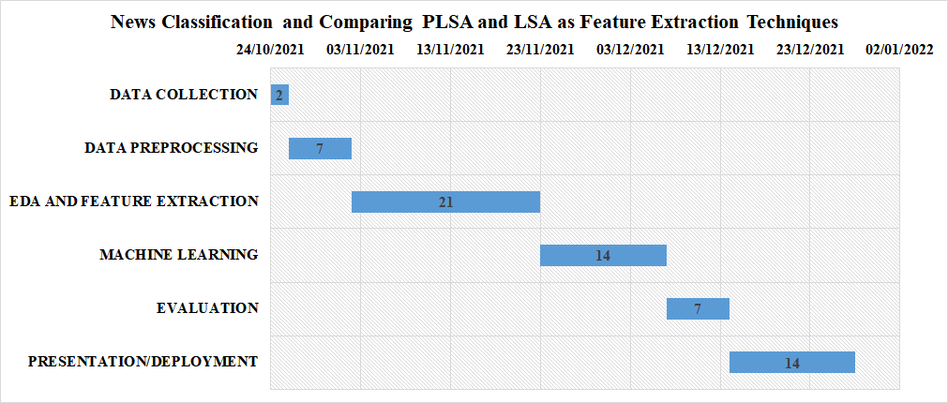
\includegraphics[scale=0.45]{gantt1.png}
                    \caption{\textbf{The gantt-chart for building the proposed system.}}
                \end{figure}
          
        \newpage
        \chapter{System Design}
        \section{System Architecture}
                This project takes the nepali texts as input and these inputs are preprocessed to generate appropritae condition to extract 
                the feature from the texts.
                Data was cleaned by removing unnecessary punctuations, emojis and symbols. After the preprocessing, words with count one were removed as well. And the given data were vectorized using TF-IDF for LSA.
                While for PLSA the document-term matrix was used to get the better representation of texts.

                \begin{figure}[h!]
                        \centering
                        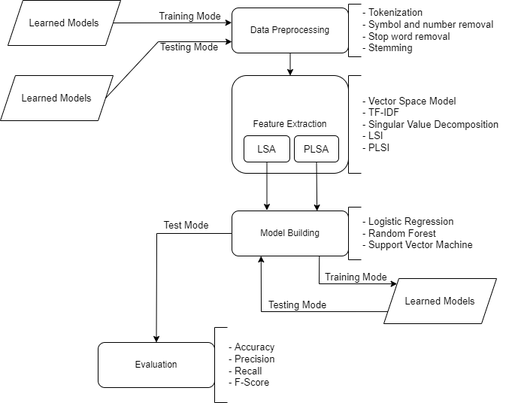
\includegraphics[scale=0.8]{system_architeture.png}
                        \caption{The architecture of the Text Classification}
                   
                \end{figure}
        \section{Process Design}
        \subsection{Data Design}
        The Nepali texts used data structure rather than relational database. In this project we used program componenet level data design technique. We can use
        different data structure like Array, List, Dictionary.

        \subsection{Class Diagram}
        The process design is as below:
        \begin{figure}[h]
            \centering
            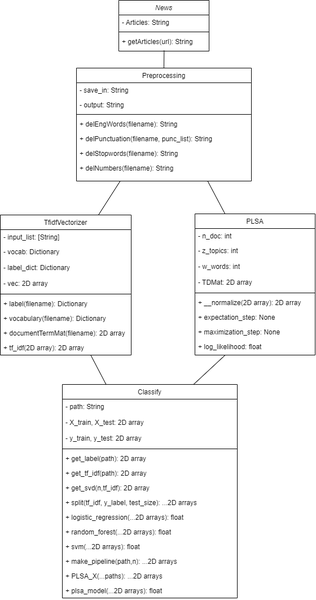
\includegraphics[scale=0.85]{class_diagram.png}
        \end{figure}

        \chapter{Implementation and Testing}
        
        \section{Implementation}
        \subsection{Tools used} Python, scikit-learn, numpy, matplotlib

        \section{Testing}
        The testing was done to find the possible flaws and the potential inefficiency of the system.

        \subsection{Unit Testing}
        Unit testing refers to the testing of every small modular components of the system, keeping them isolated from other modules.
        Here we mention testing result of the various part of the system. In unit testing, we design the whole system in modularized pattern and 
        each module was tested. 
        Test cases of system during feature extraction,

        E.g.,

            For document-term matrix we can see that: 
            \begin{figure}[h]
                \centering
                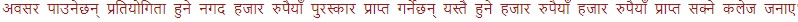
\includegraphics[scale=0.7]{testText.jpg}
                \caption{Text for testing for document term matrix}
            \end{figure}
            \begin{figure}[h]
                \centering
                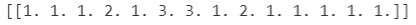
\includegraphics{docTerm.jpg}
                \caption{ Document term matrix for the given test text}
            \end{figure}


        \subsection{System Testing}
        In this testing phase our system as a whole was tested. Every individual component was integrated and tested.

        \subsection{Evaluation of the Model}
        Three different evaluation technique like: precision, recall and f-score were used.
        They are defined as follows:
        \begin{figure}[h]
            \centering
            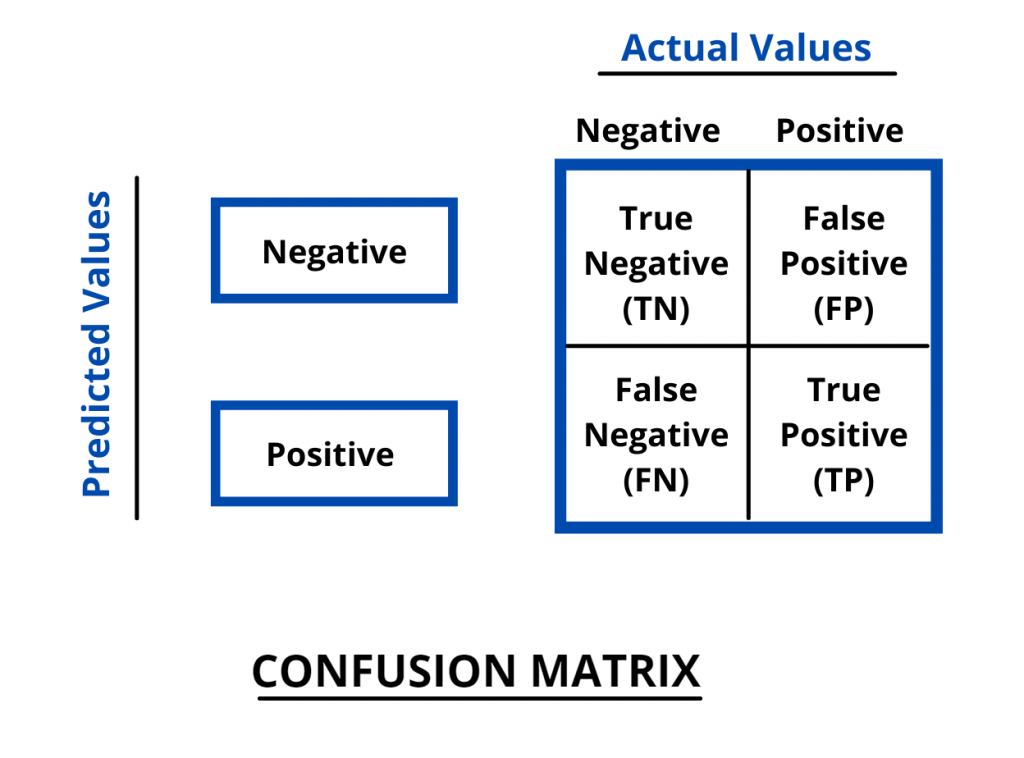
\includegraphics[scale=0.4]{confusion_matrix.png}
            \caption{Confusion matrix}
        \end{figure}
            \begin{center}
                \begin{equation}
                    Accuracy = \frac{TP + TN }{TP +  + TN + FN}
                \end{equation}
                \begin{equation}
                    Precision = \frac{TP}{TP + FP}
                \end{equation}
                \begin{equation}
                    Recall= \frac{TP}{TP + FN}
                \end{equation}
                \begin{equation}
                    F-measure= \frac{2 * (Precision * Recall)}{Precision +  Recall}
                \end{equation}
            \end{center}



            \begin{figure}[h]
                \begin{minipage}{0.48\textwidth}
                  \centering
                  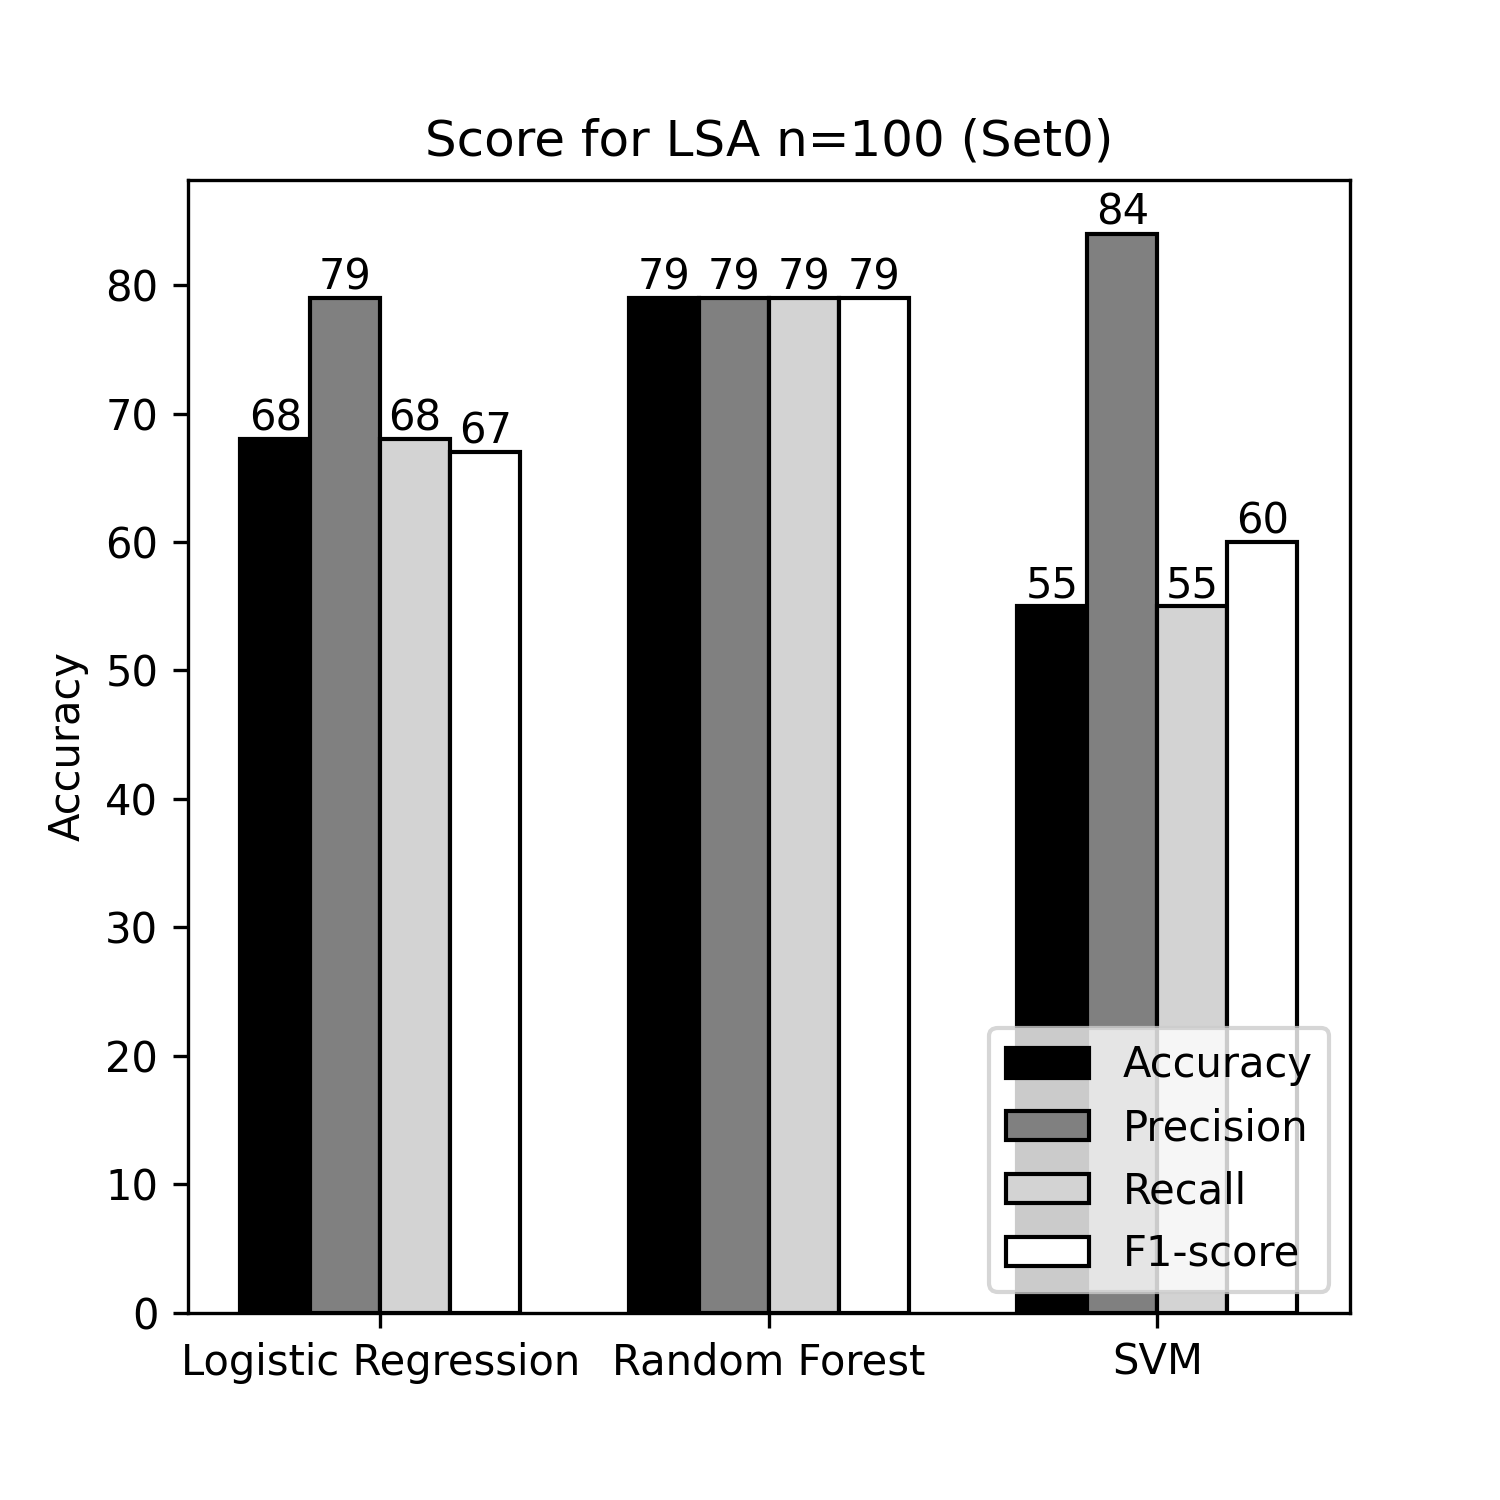
\includegraphics[scale=0.55]{plots/Score for LSA n=100 (Set0).png}
                  \caption{Score for LSA n=100 (Set0)}\label{Fig:typo1}
                \end{minipage}\hfill
                \begin{minipage}{0.48\textwidth}
                  \centering
                  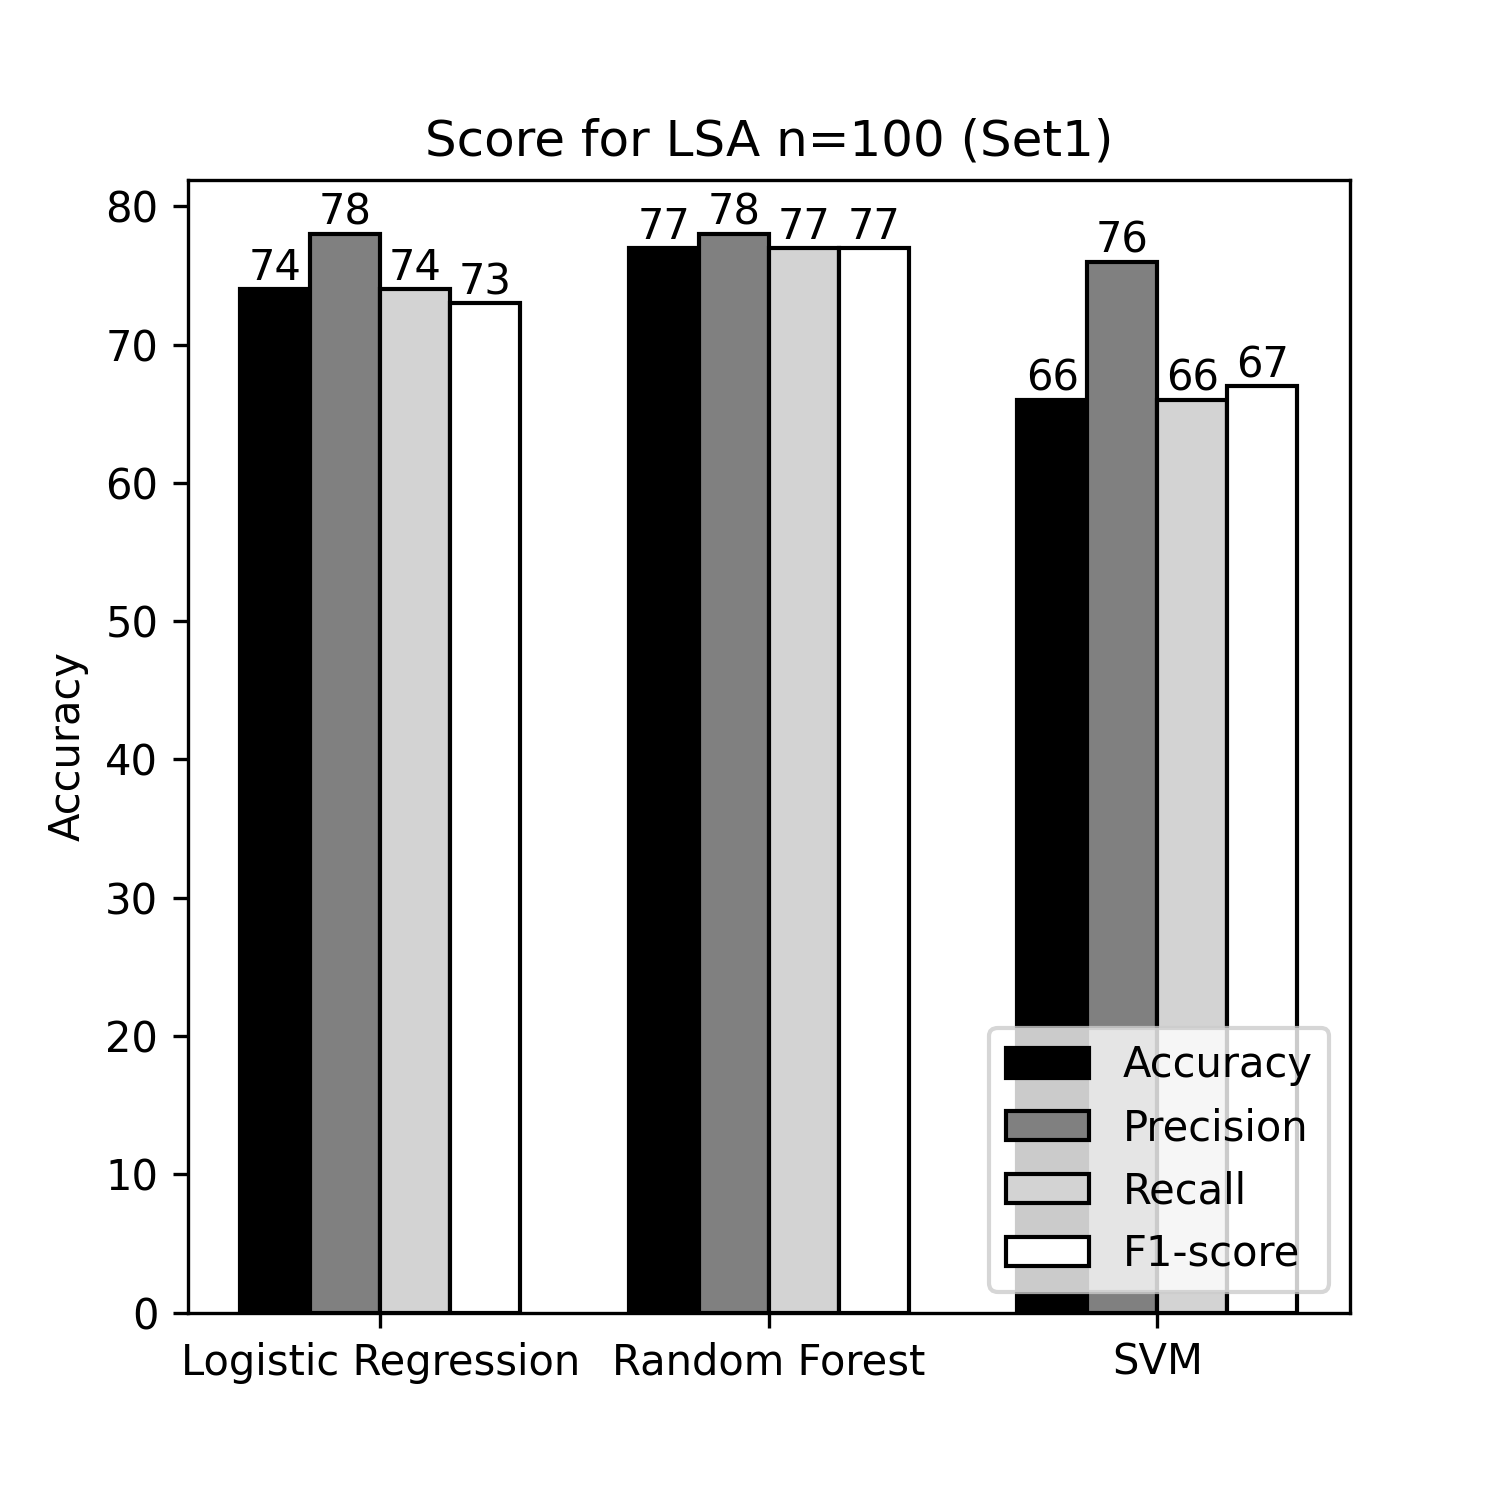
\includegraphics[scale=0.55]{plots/Score for LSA n=100 (Set1).png}
                  \caption{Score for LSA n=100 (Set1)}\label{Fig:tyo2}
                \end{minipage}
             \end{figure}

             \begin{figure}[h]
                \begin{minipage}{0.48\textwidth}
                  \centering
                  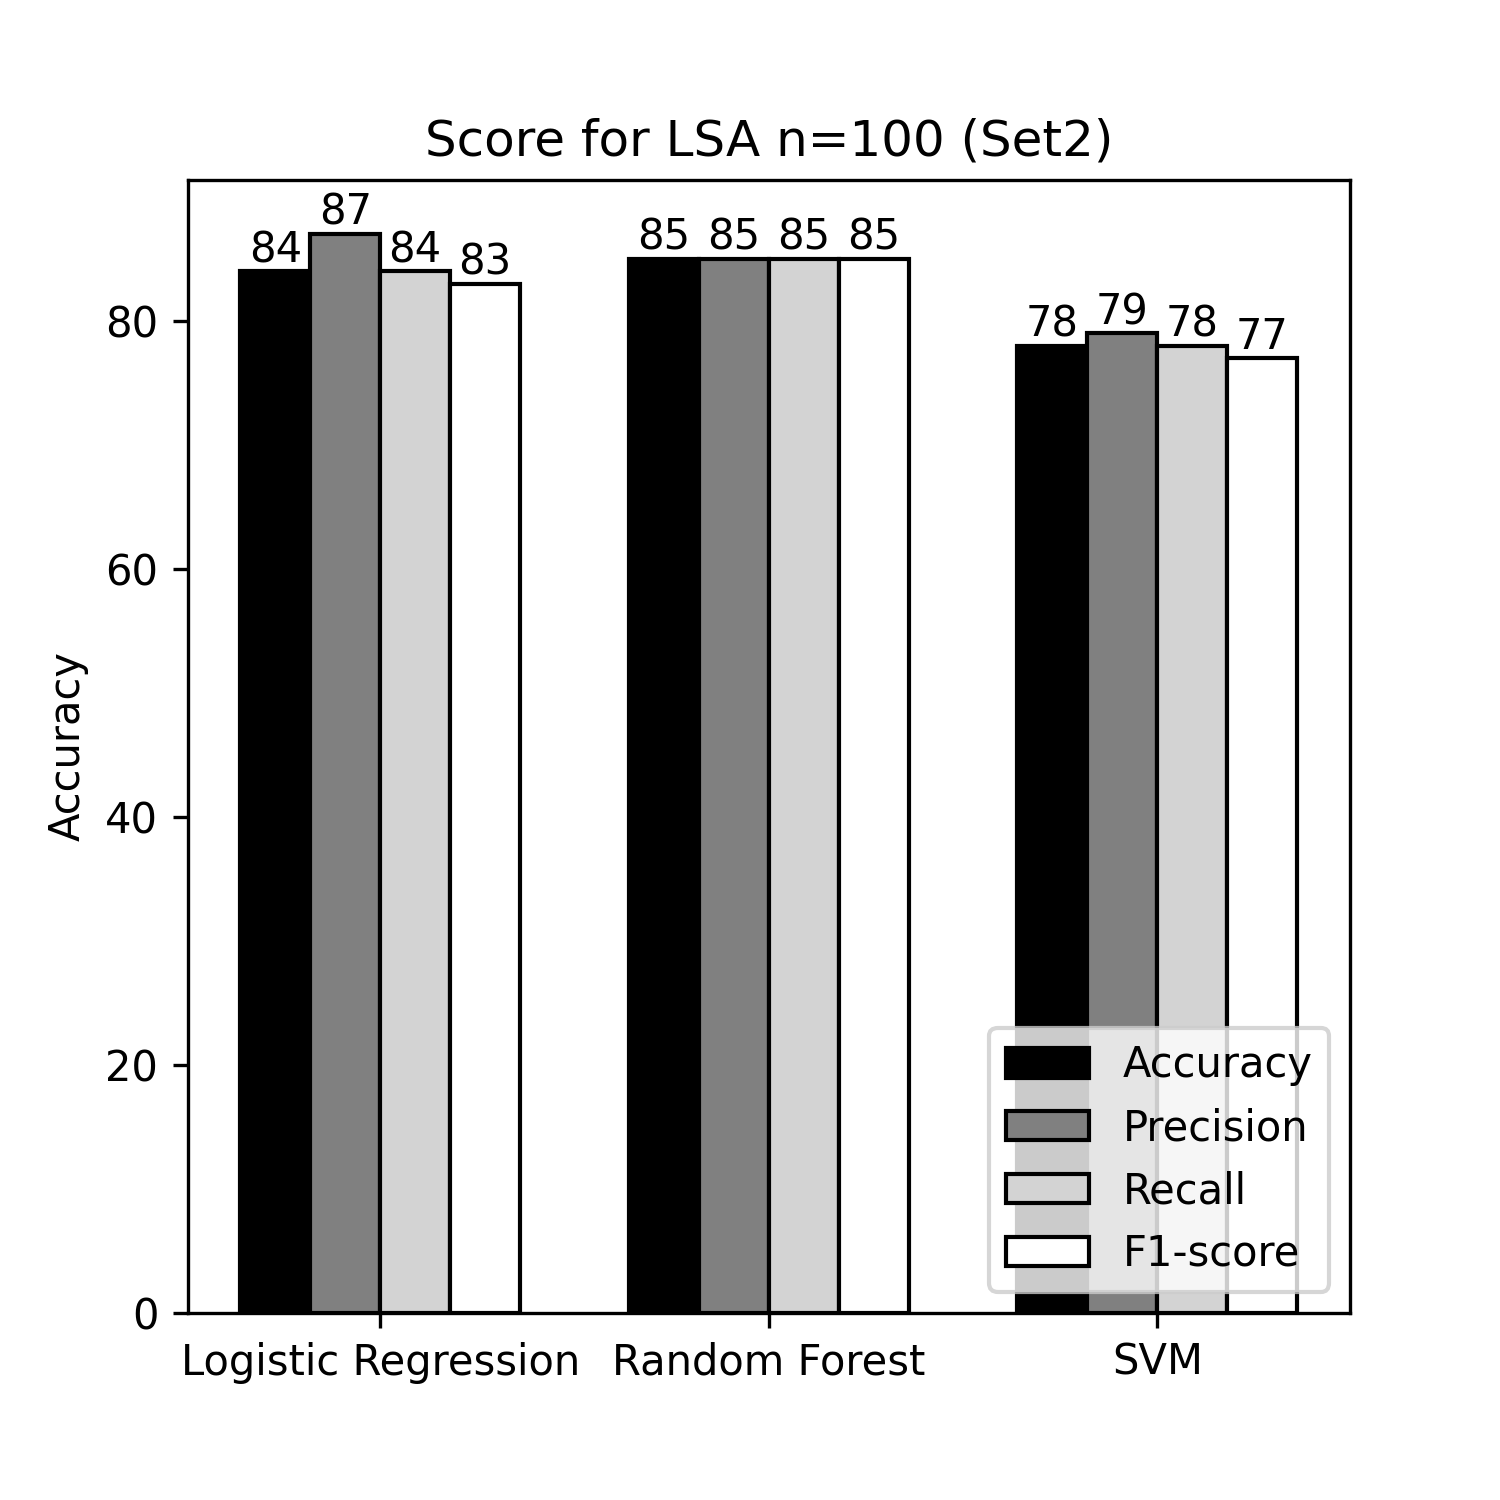
\includegraphics[scale=0.55]{plots/Score for LSA n=100 (Set2).png}
                  \caption{Score for LSA n=100 (Set2)}\label{Fig:typo1}
                \end{minipage}\hfill
                \begin{minipage}{0.48\textwidth}
                  \centering
                  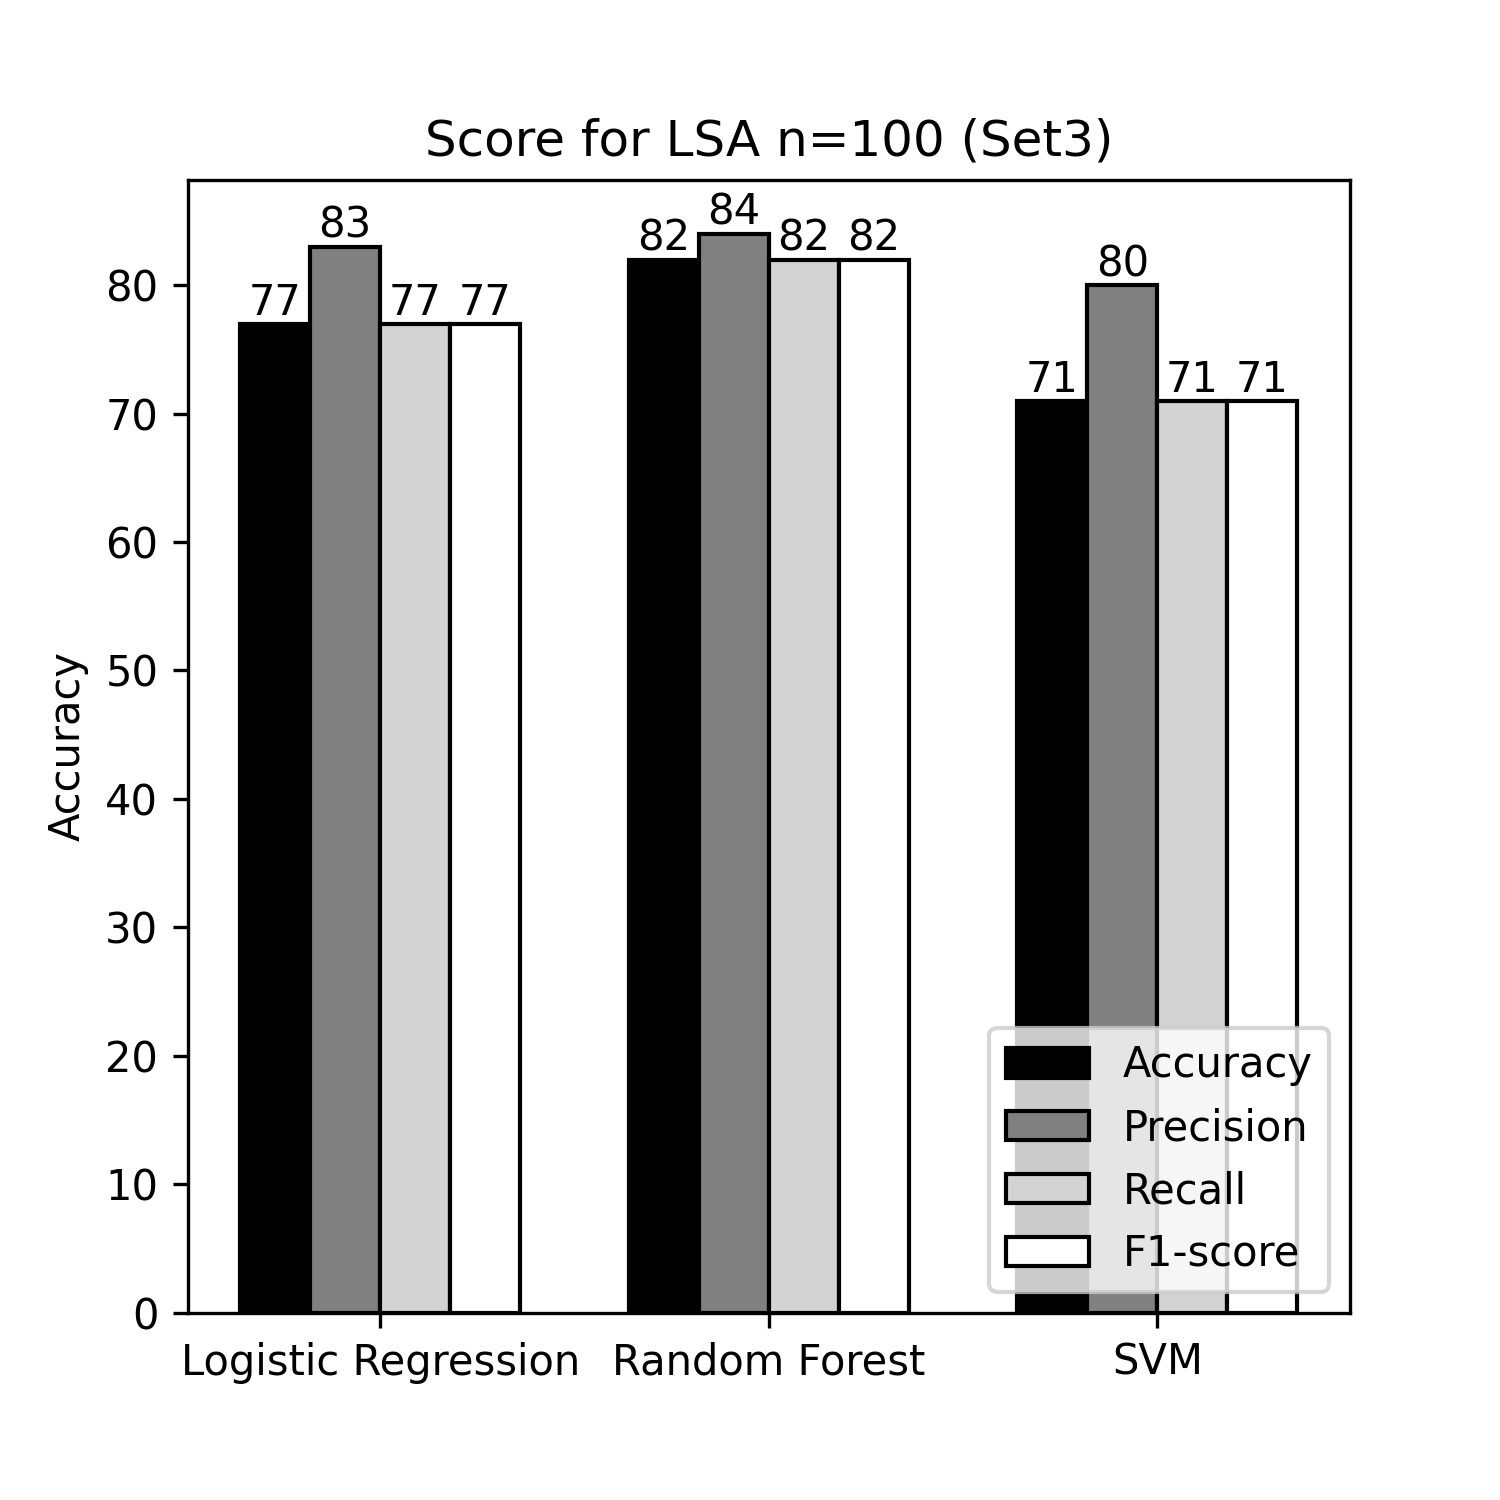
\includegraphics[scale=0.55]{plots/Score for LSA n=100 (Set3).png}
                  \caption{Score for LSA n=100 (Set3)}\label{Fig:typo2}
                \end{minipage}
             \end{figure}

             In the first experiment, we lowered the latent-concept to 100. And then, different sized dataset of 1600, 1200, 1000, and 600 were 
             trained and evaluated. The figure 5.4 to 5.7 explains the evaluation metrics for it. It showed random forest algorithm 
             was more consistent which made sense as it is an ensemble techinque. 


             
             \begin{figure}[!htb]
                \begin{minipage}{0.48\textwidth}
                  \centering
                  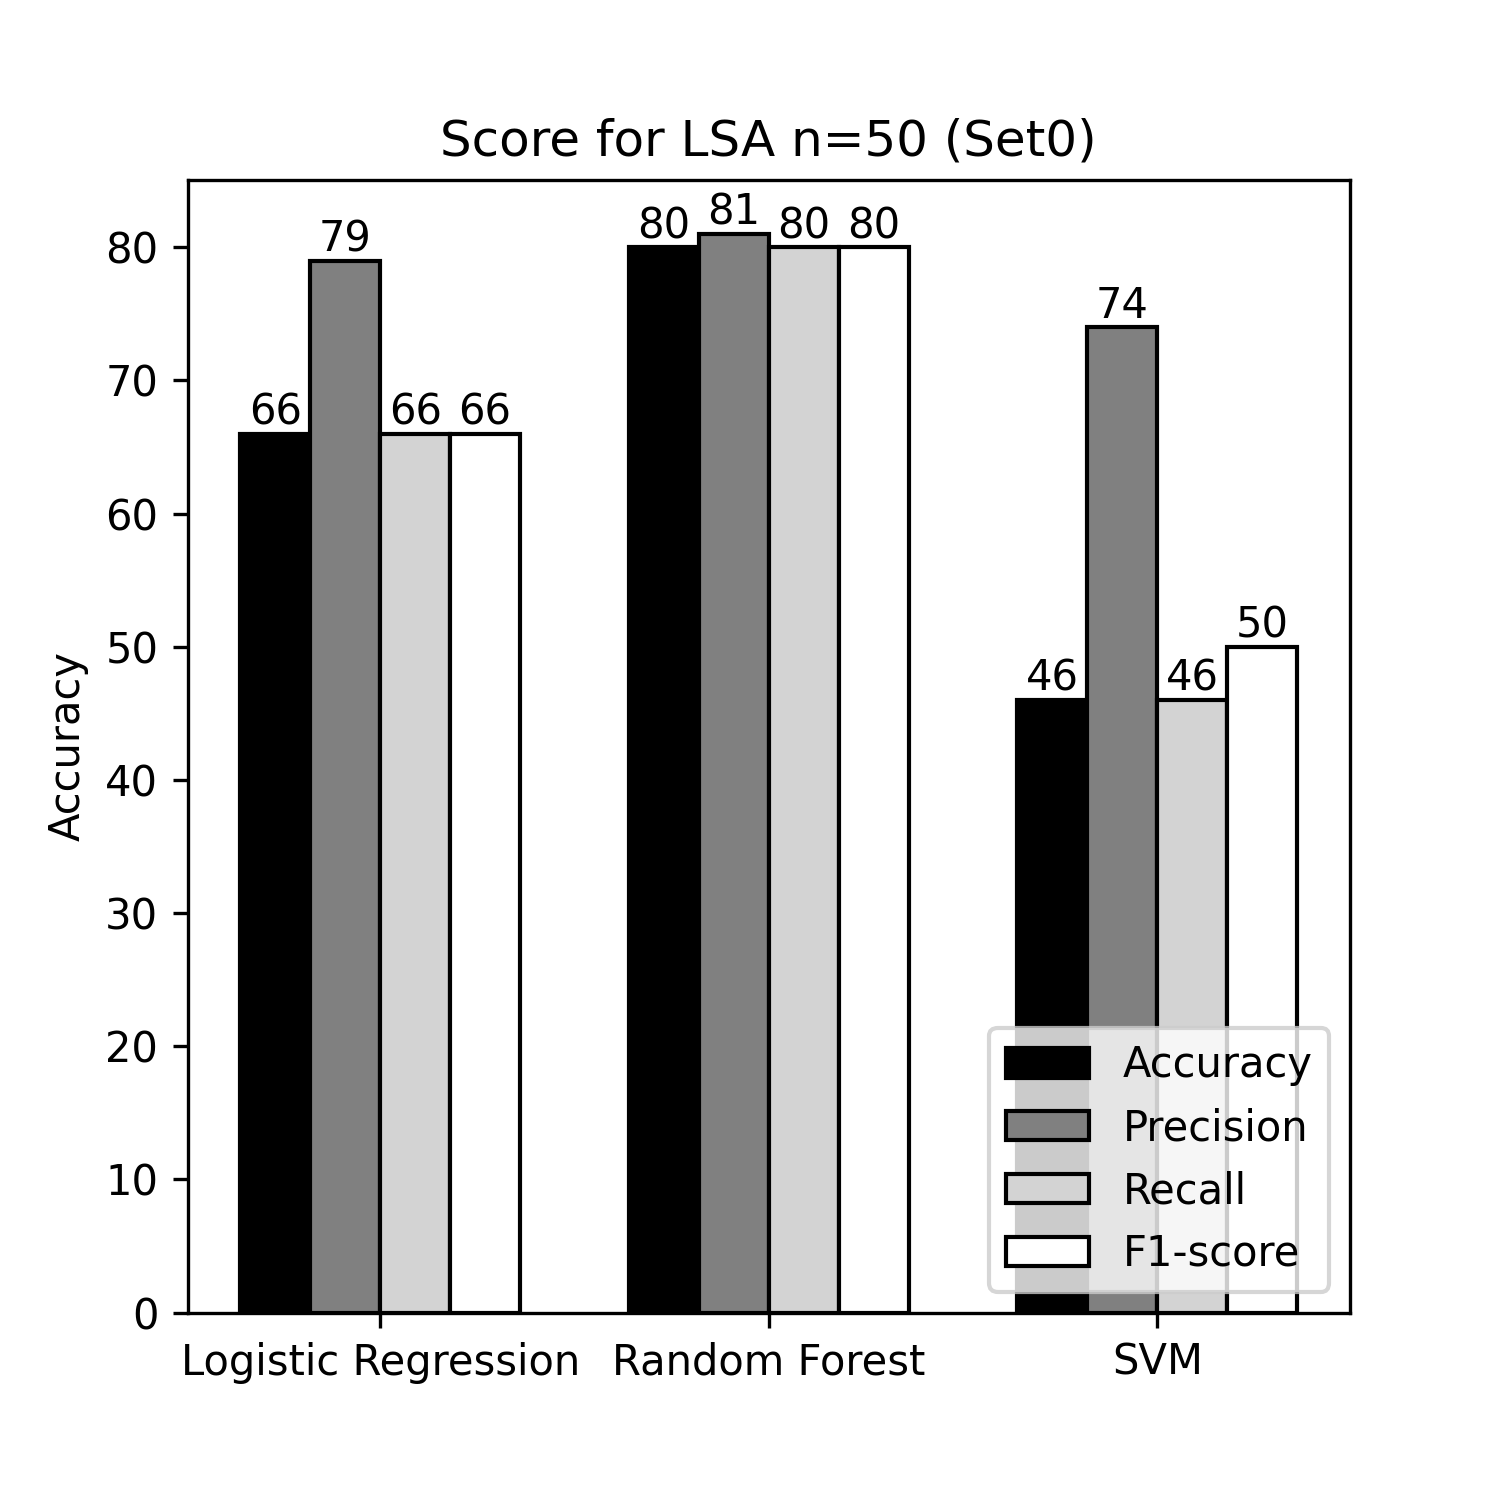
\includegraphics[scale=0.55]{plots/Score for LSA n=50 (Set0).png}
                  \caption{Score for LSA n=50 (Set0)}\label{Fig:typo1}
                \end{minipage}\hfill
                \begin{minipage}{0.48\textwidth}
                  \centering
                  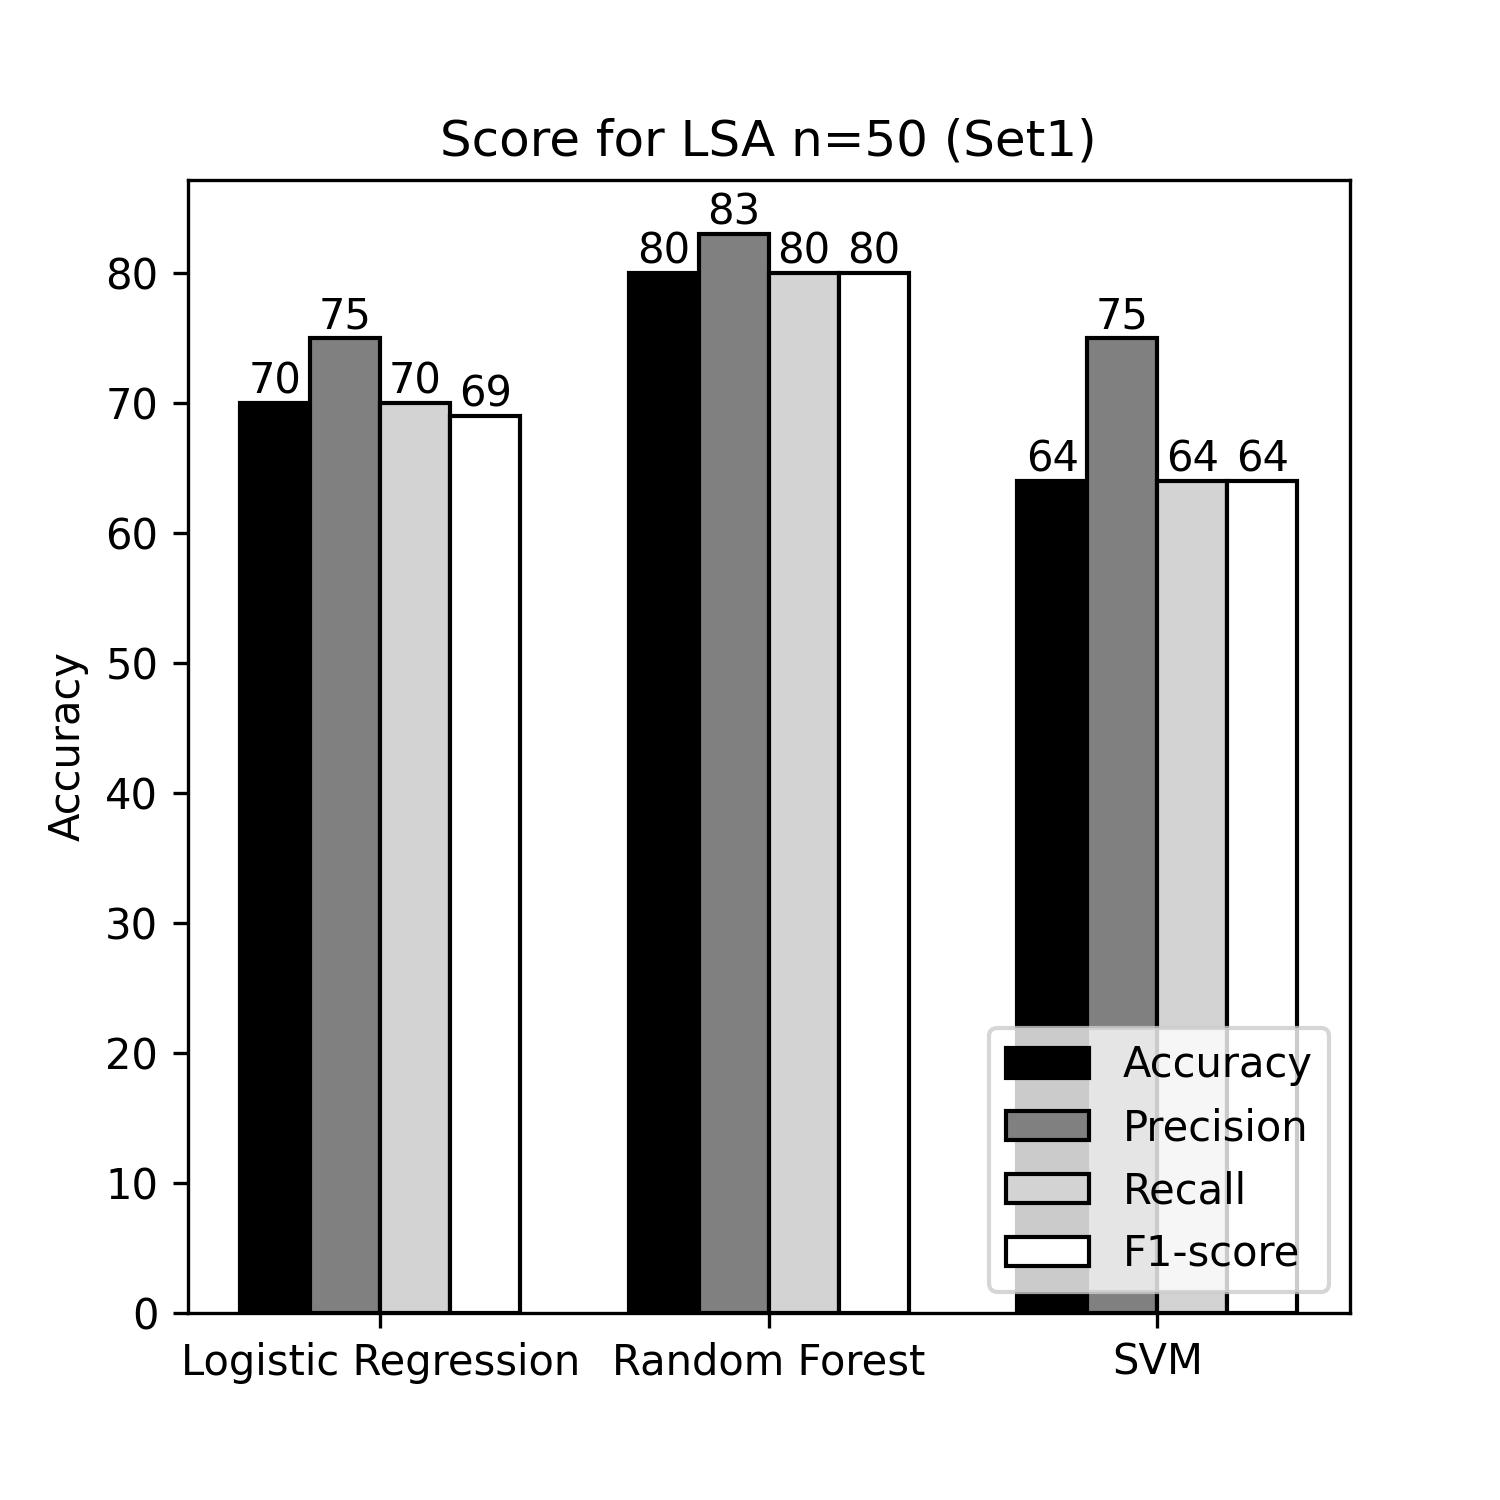
\includegraphics[scale=0.55]{plots/Score for LSA n=50 (Set1).png}
                  \caption{Score for LSA n=50 (Set1)}\label{Fig:typo2}
                \end{minipage}
             \end{figure}


             \begin{figure}[!htb]
                \begin{minipage}{0.48\textwidth}
                  \centering
                  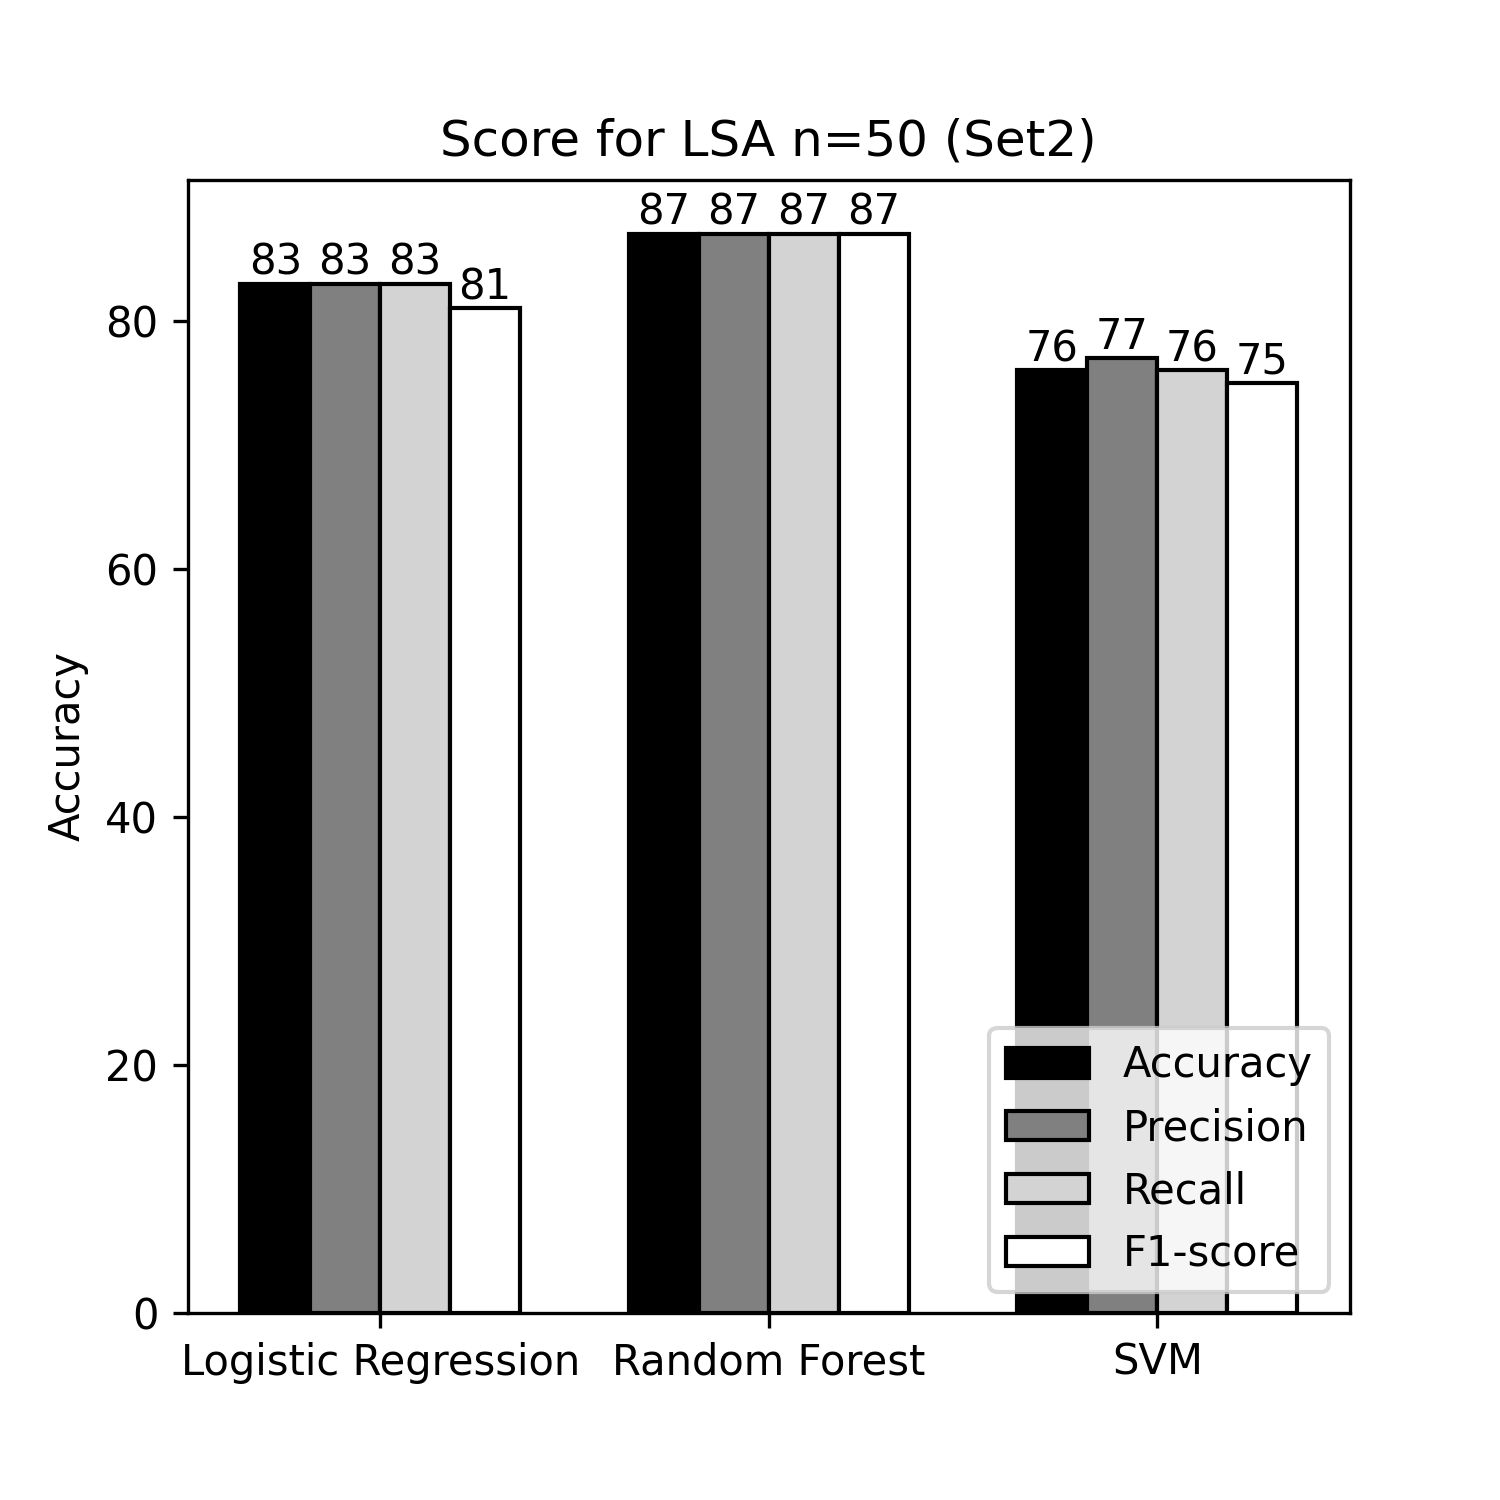
\includegraphics[scale=0.55]{plots/Score for LSA n=50 (Set2).png}
                  \caption{Score for LSA n=50 (Set2)}\label{Fig:typo1}
                \end{minipage}\hfill
                \begin{minipage}{0.48\textwidth}
                  \centering
                  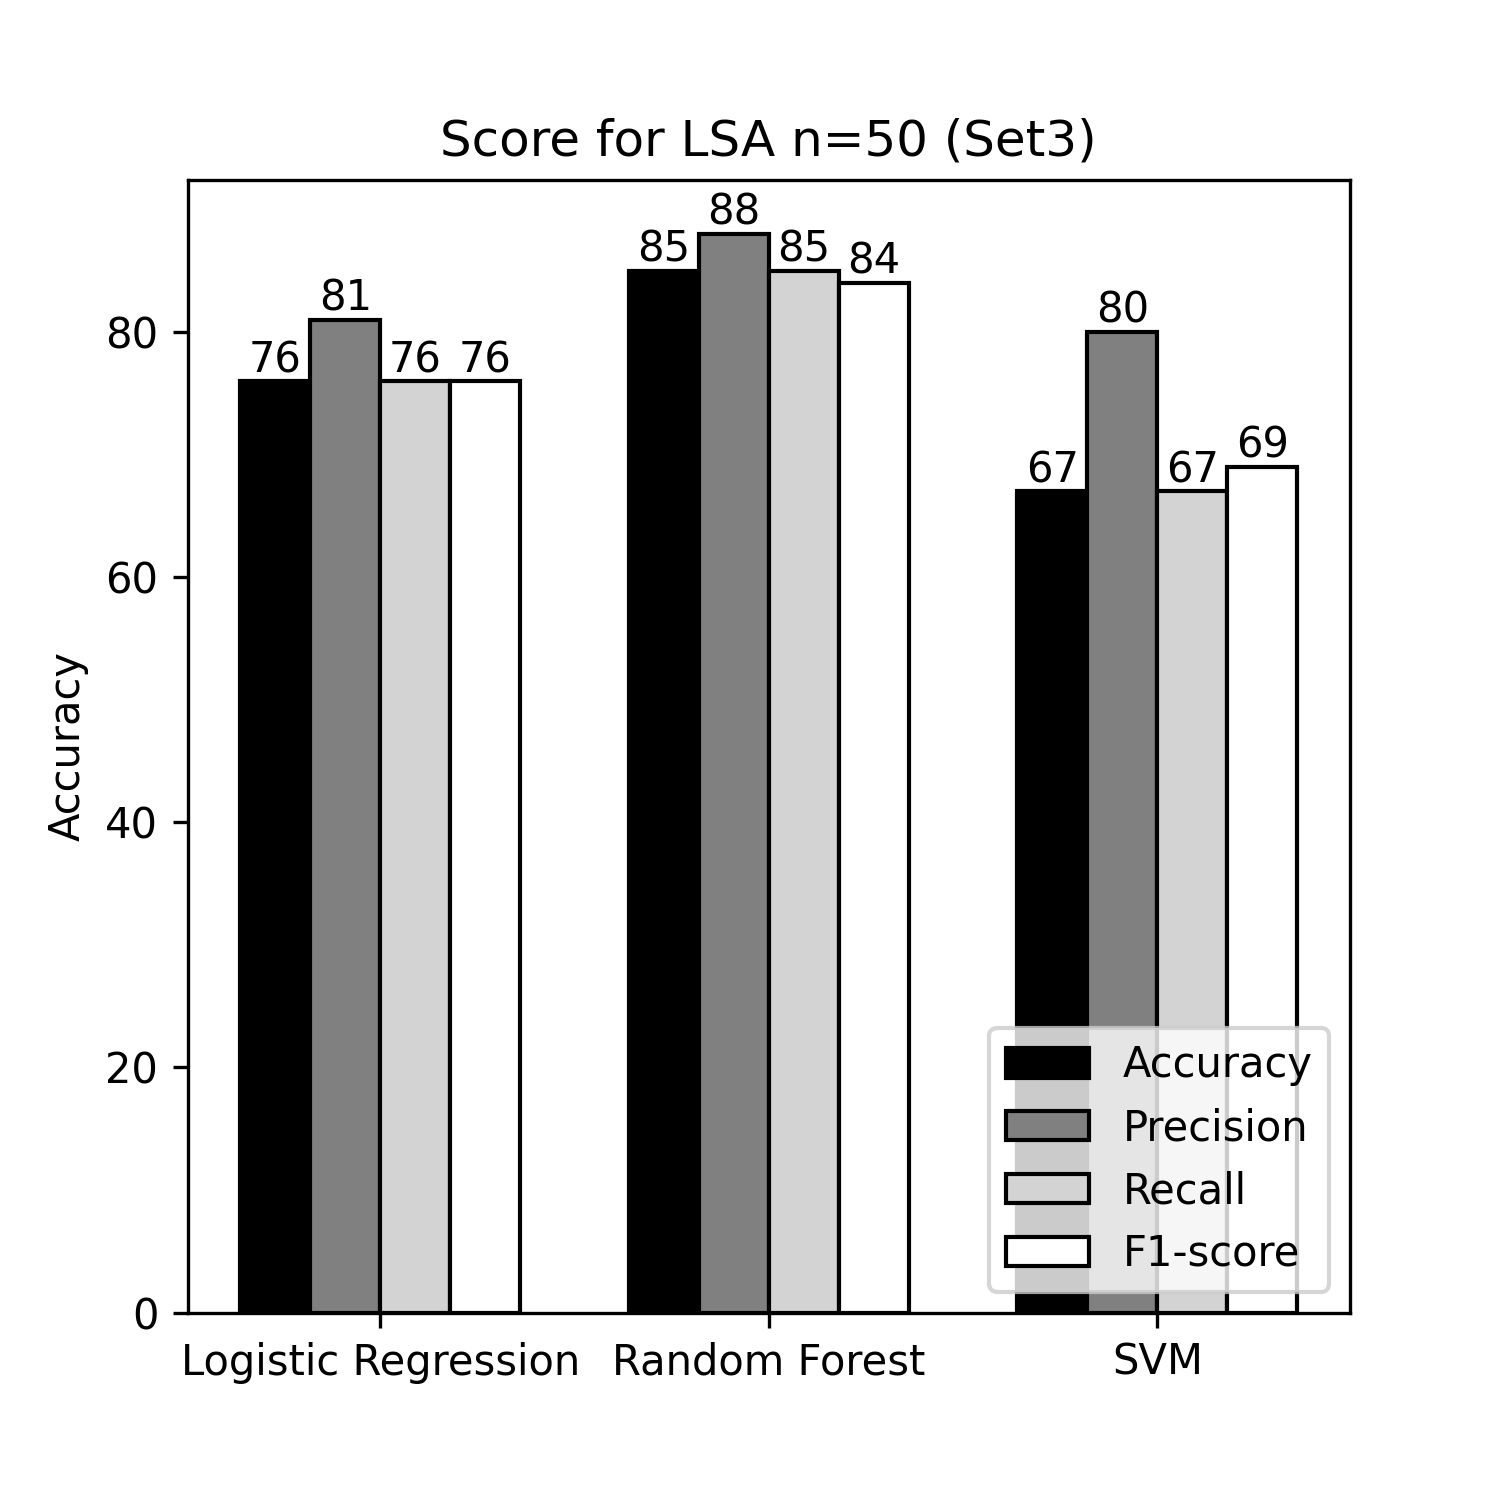
\includegraphics[scale=0.55]{plots/Score for LSA n=50 (Set3).png}
                  \caption{Score for LSA n=50 (Set3)}\label{Fig:typo2}
                \end{minipage}
             \end{figure}


             In the second experiment, we lowered the latent-concept to 50 which was evaluated on the same sets of data as befores. The figure 5.8 to 5.11 explains the evaluation metrics for it. 
             Random forest had slight improvement in all evaluation scores. We can attribute this to lowerered sparsity of matrix.

             


             \begin{figure}[!htb]
                \begin{minipage}{0.48\textwidth}
                  \centering
                  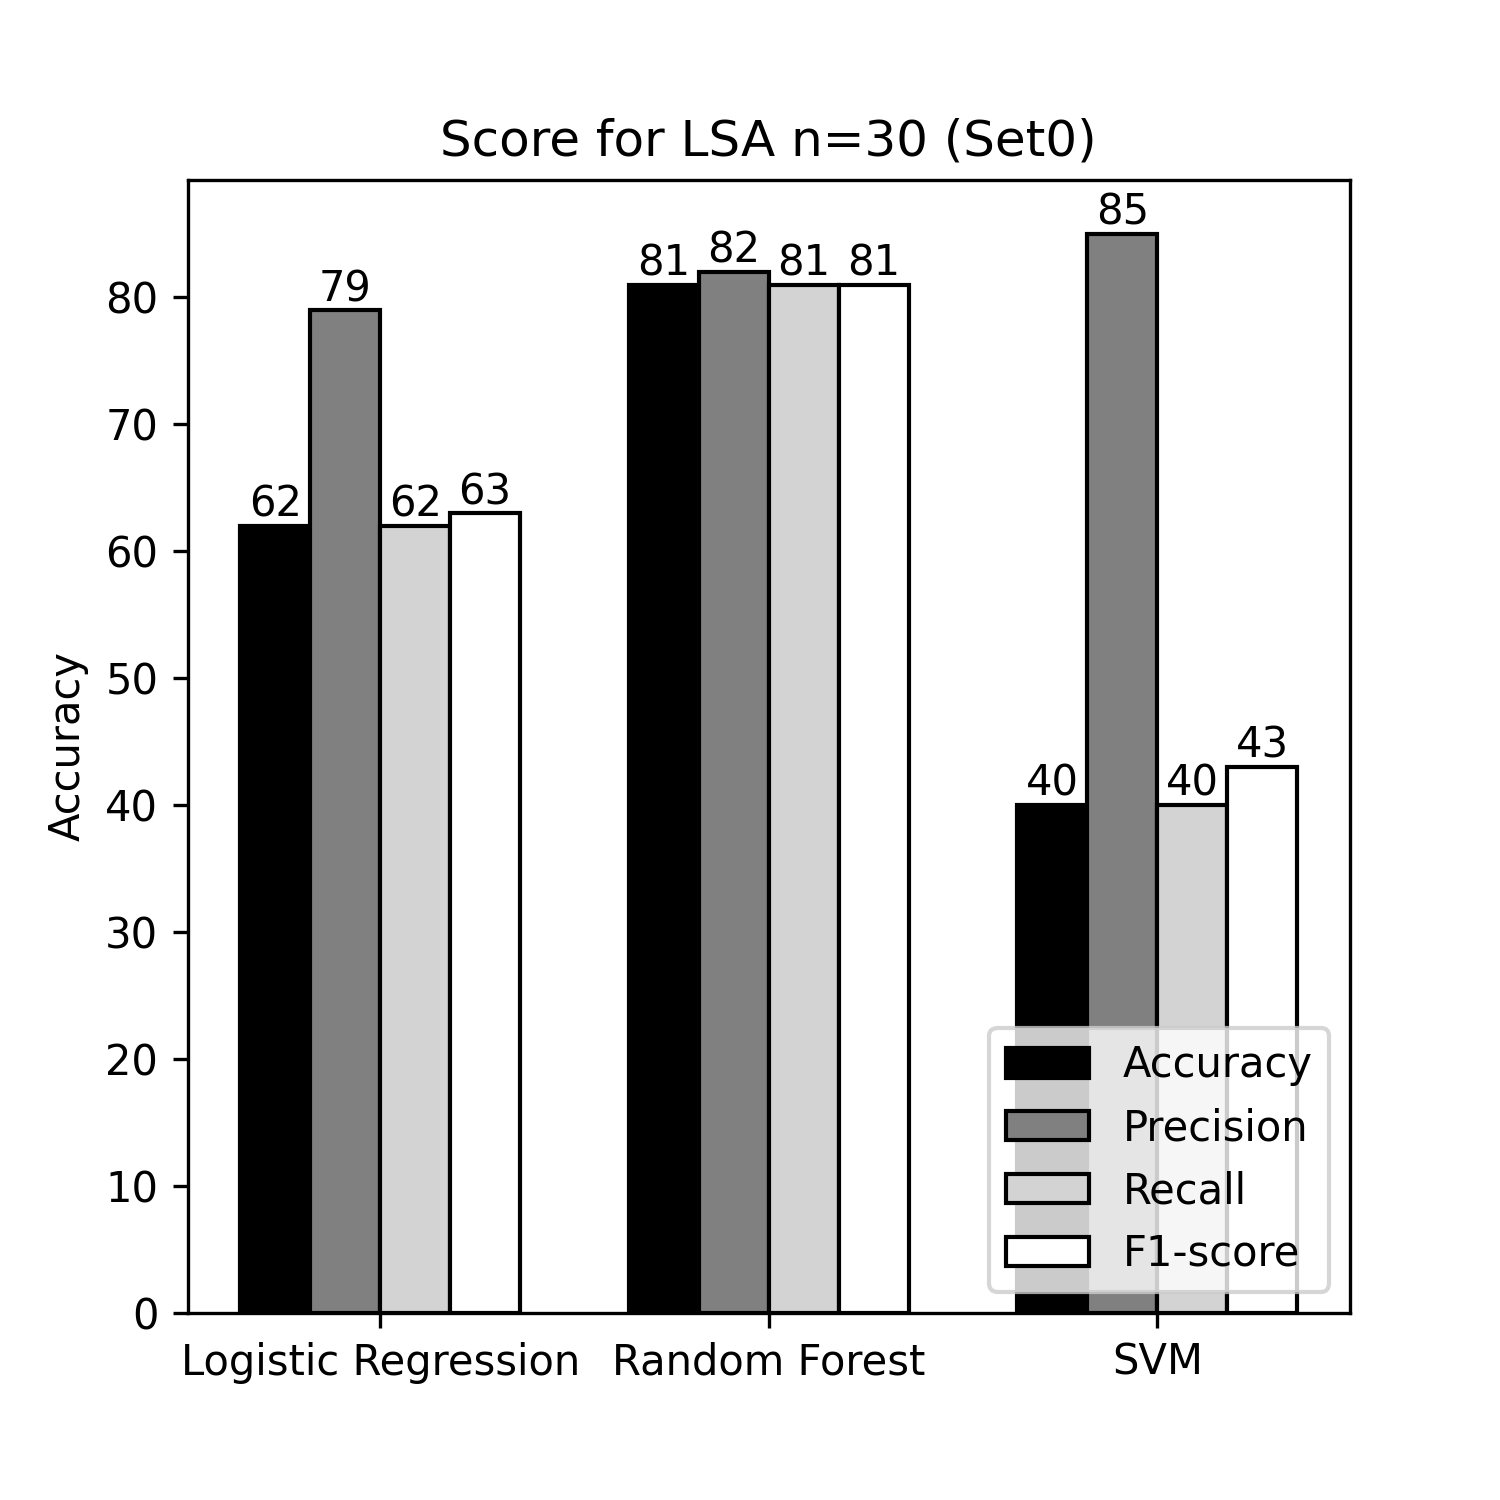
\includegraphics[scale=0.55]{plots/Score for LSA n=30 (Set0).png}
                  \caption{Score for LSA n=30 (Set0)}\label{Fig:typo1}
                \end{minipage}\hfill
                \begin{minipage}{0.48\textwidth}
                  \centering
                  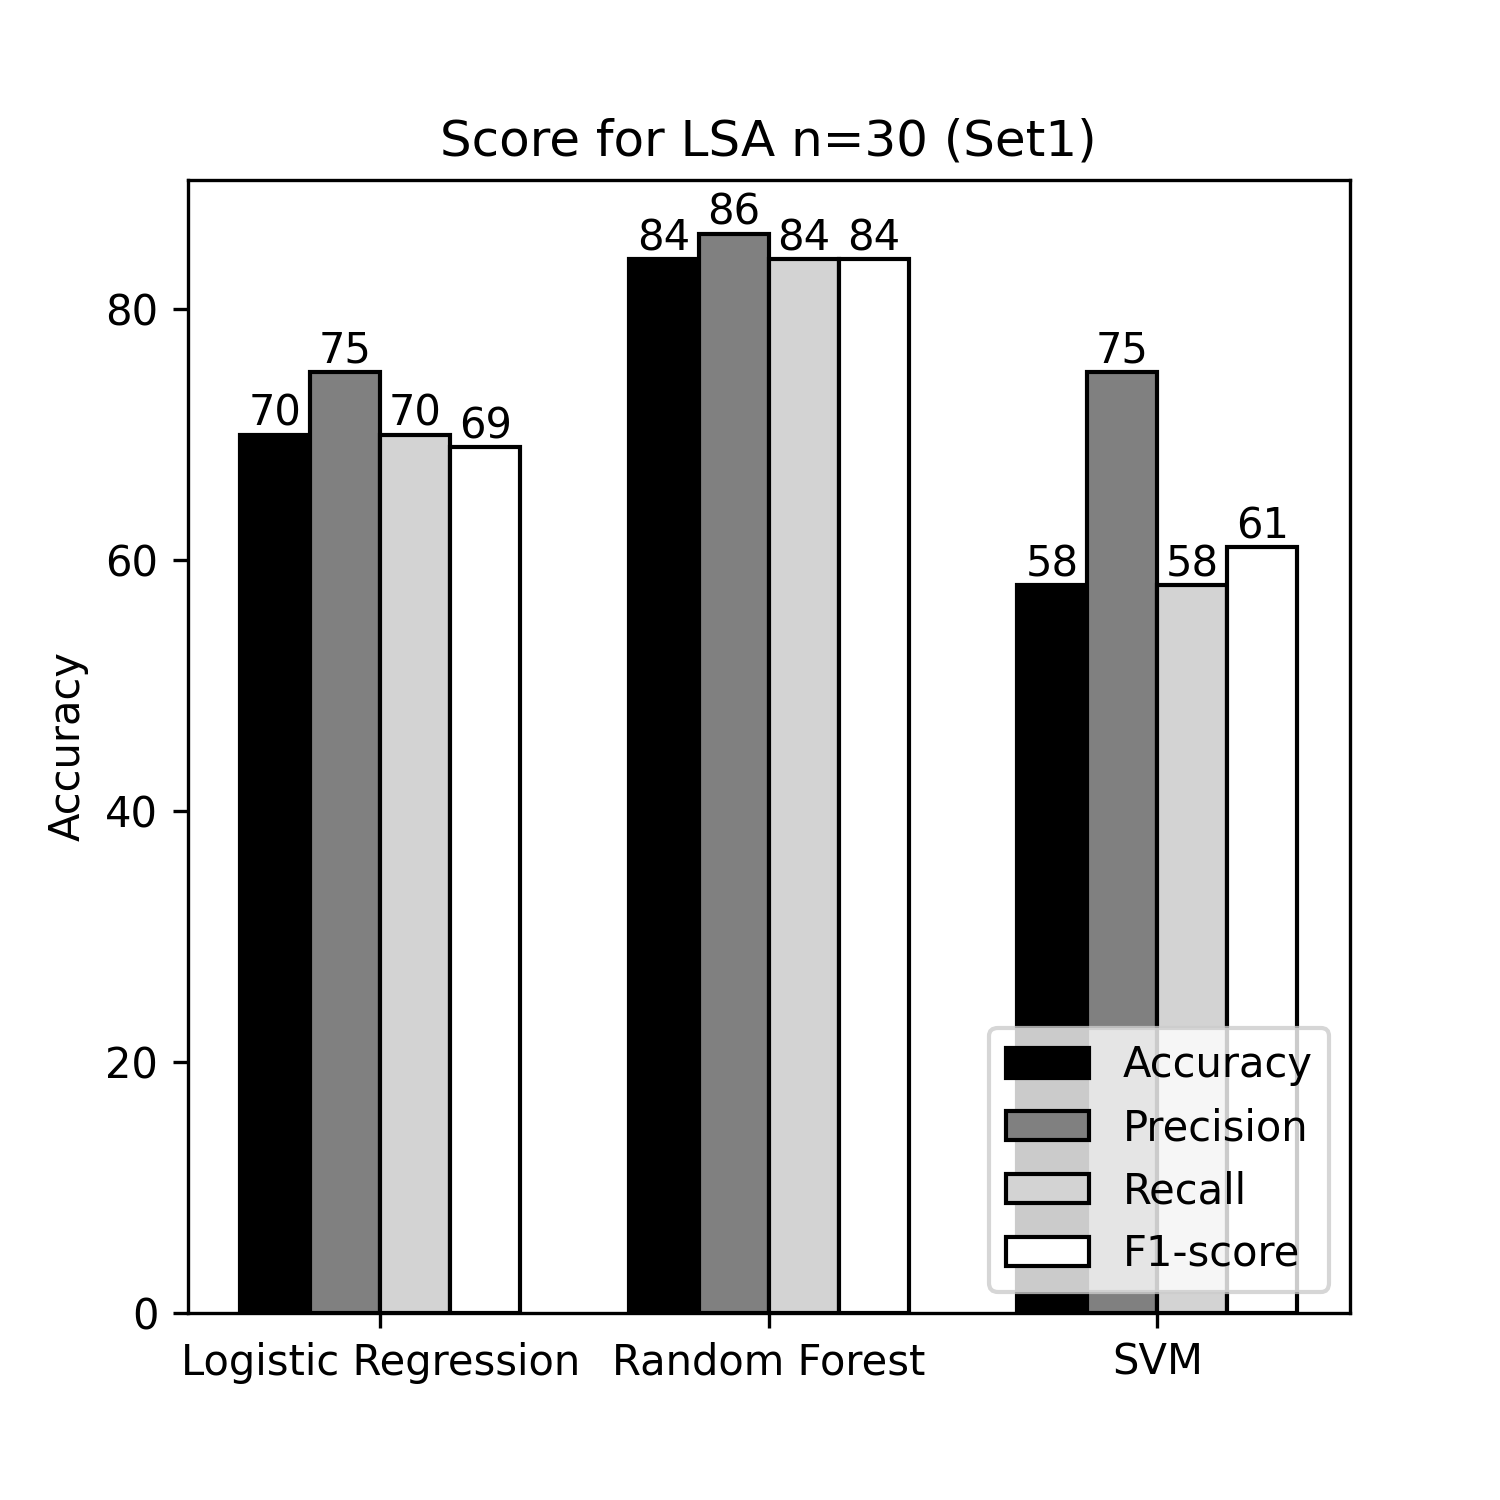
\includegraphics[scale=0.55]{plots/Score for LSA n=30 (Set1).png}
                  \caption{Score for LSA n=30 (Set1)}\label{Fig:typo2}
                \end{minipage}
             \end{figure}

             \begin{figure}[!htb]
                \begin{minipage}{0.48\textwidth}
                  \centering
                  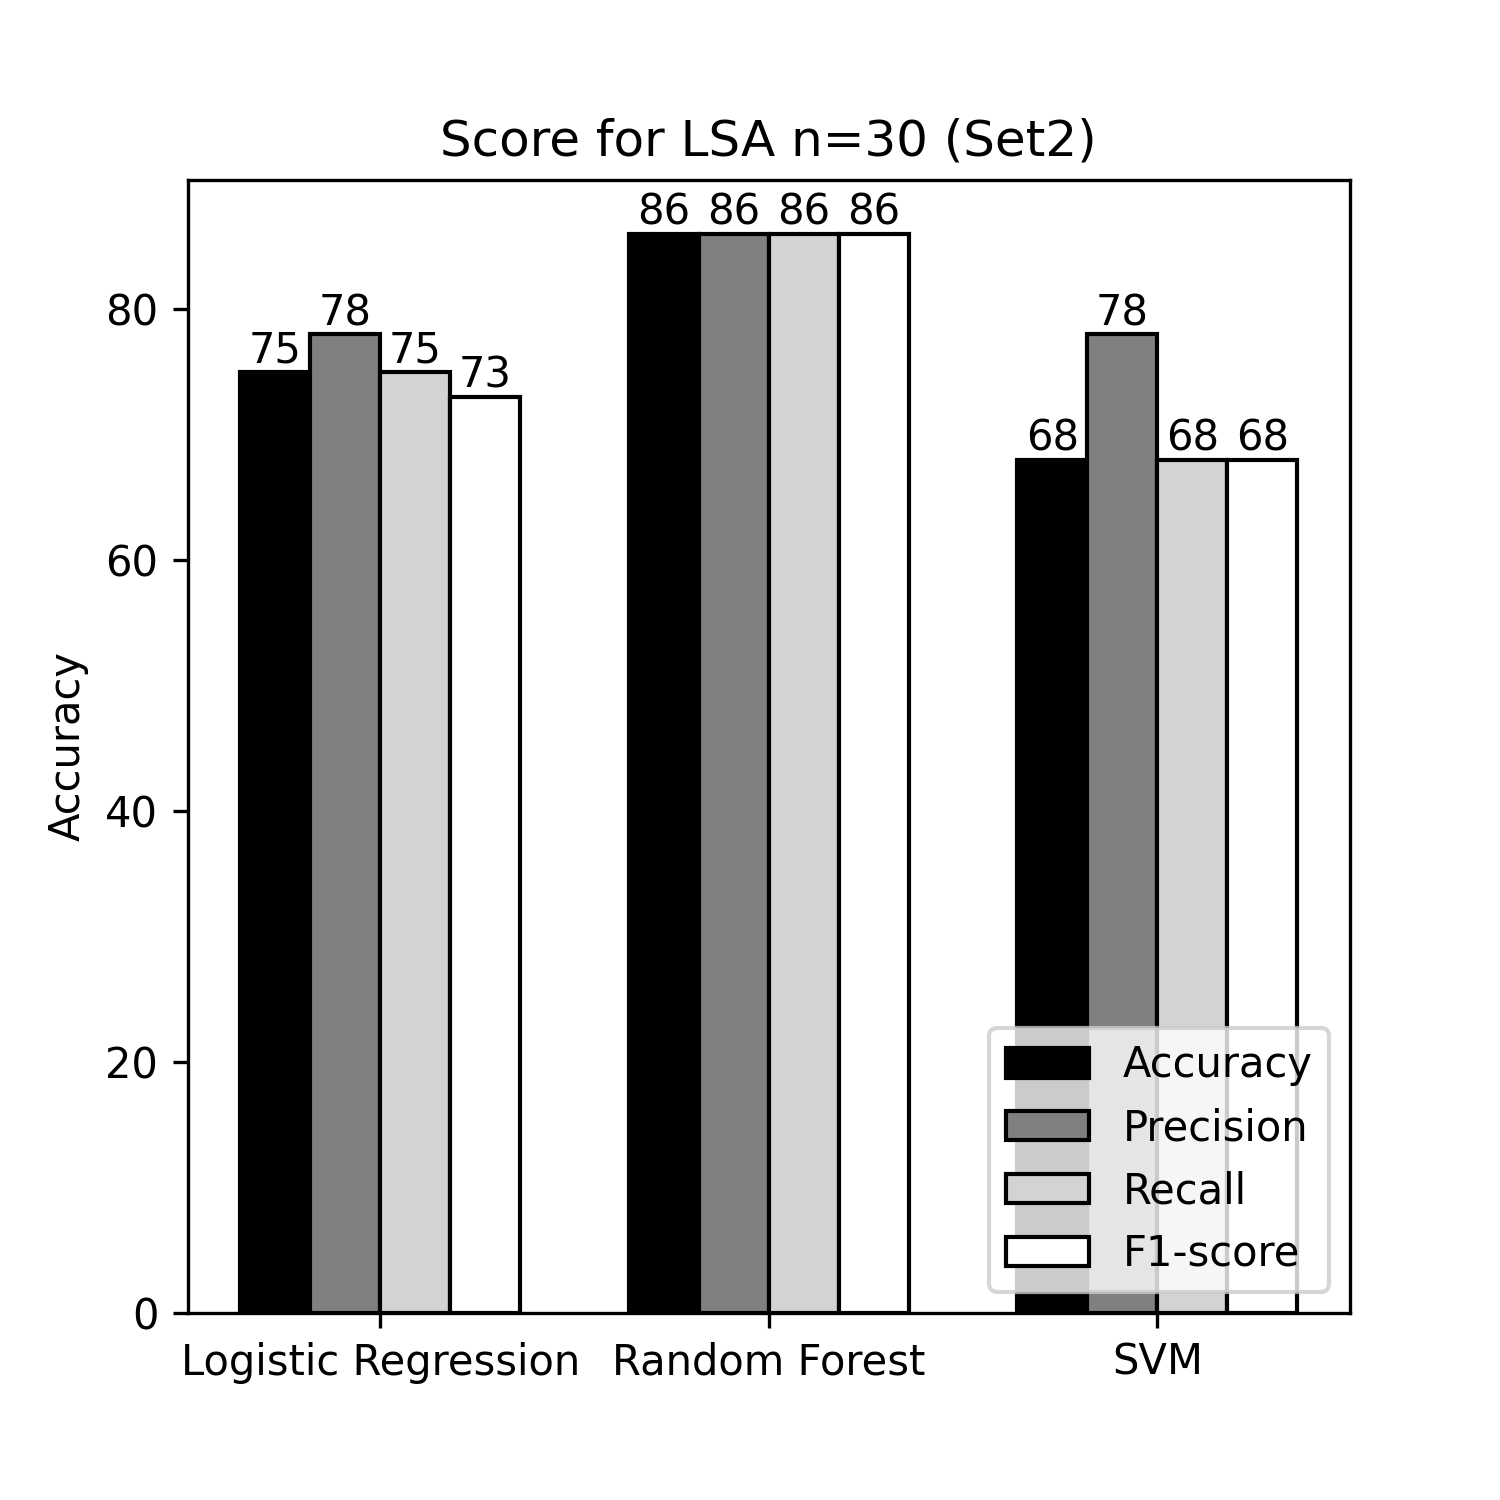
\includegraphics[scale=0.55]{plots/Score for LSA n=30 (Set2).png}
                  \caption{Score for LSA n=30 (Set2)}\label{Fig:typo1}
                \end{minipage}\hfill
                \begin{minipage}{0.48\textwidth}
                  \centering
                  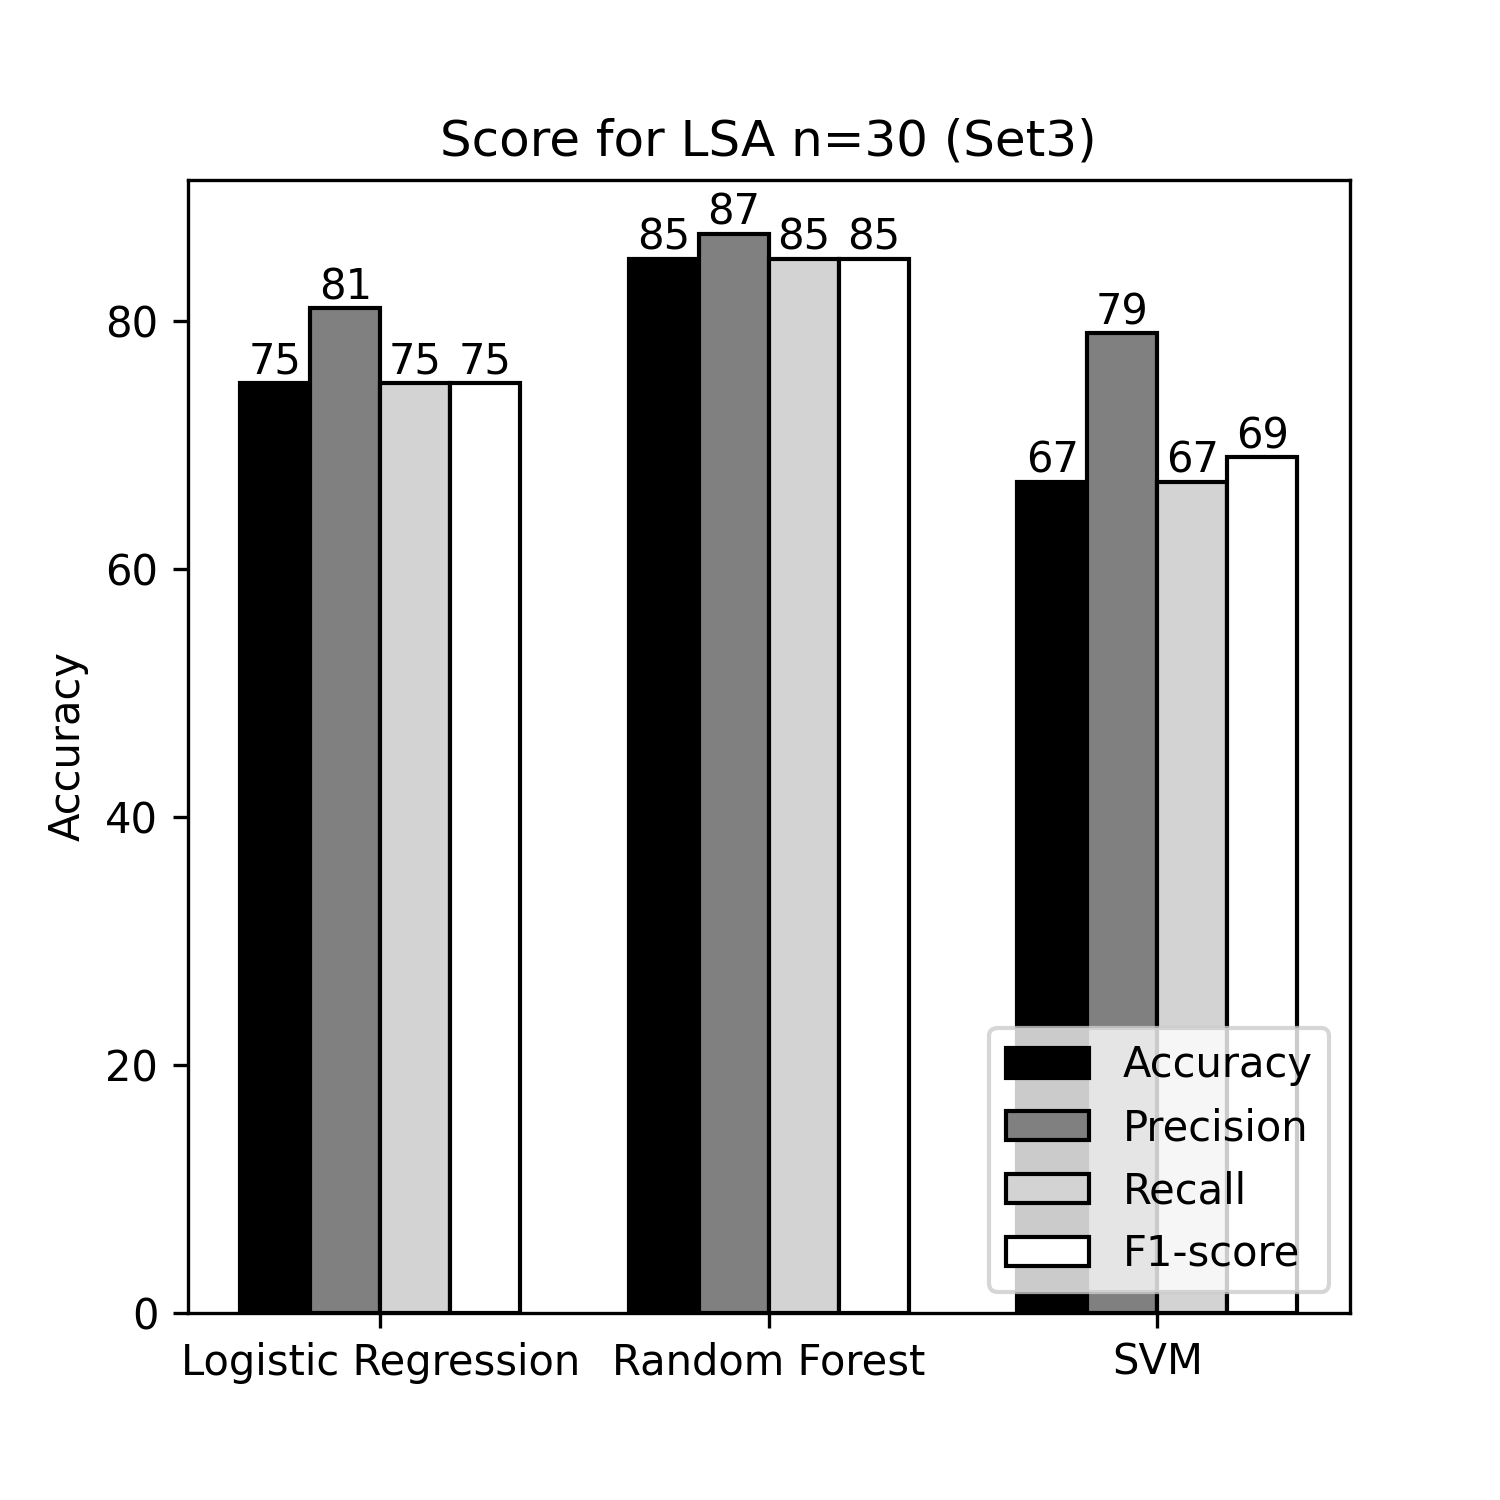
\includegraphics[scale=0.55]{plots/Score for LSA n=30 (Set3).png}
                  \caption{Score for LSA n=30 (Set3)}\label{Fig:typo2}
                \end{minipage}
             \end{figure}

             Like in the previous experiment, SVM and Logisitic Regression fall behind significantly compared to random forest and scores for Random Forest was highest.
             30 might be the optimal choice for feature extraction.


             \begin{figure}[!htb]
                \begin{minipage}{0.48\textwidth}
                  \centering
                  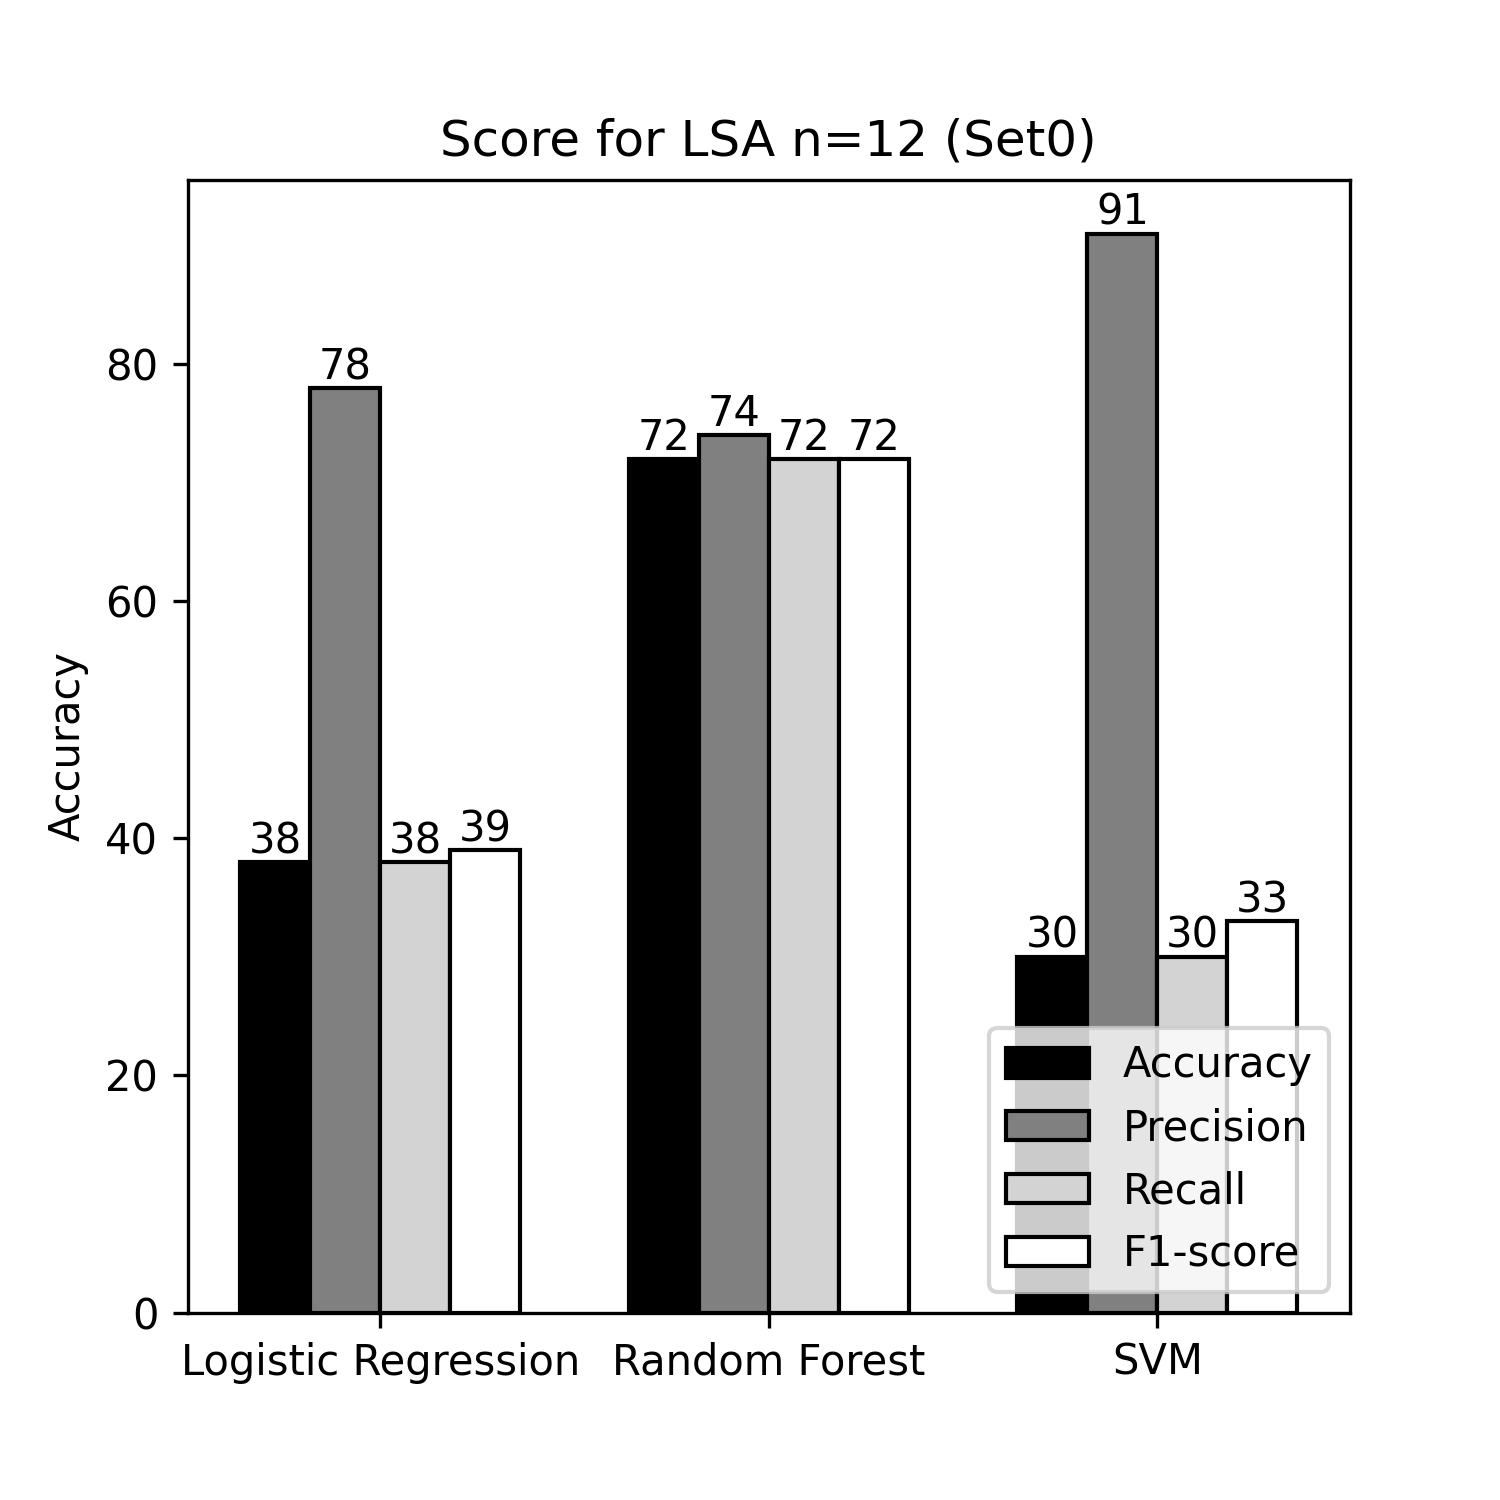
\includegraphics[scale=0.55]{plots/Score for LSA n=12 (Set0).png}
                  \caption{Score for LSA n=12 (Set0)}\label{Fig:typo1}
                \end{minipage}\hfill
                \begin{minipage}{0.48\textwidth}
                  \centering
                  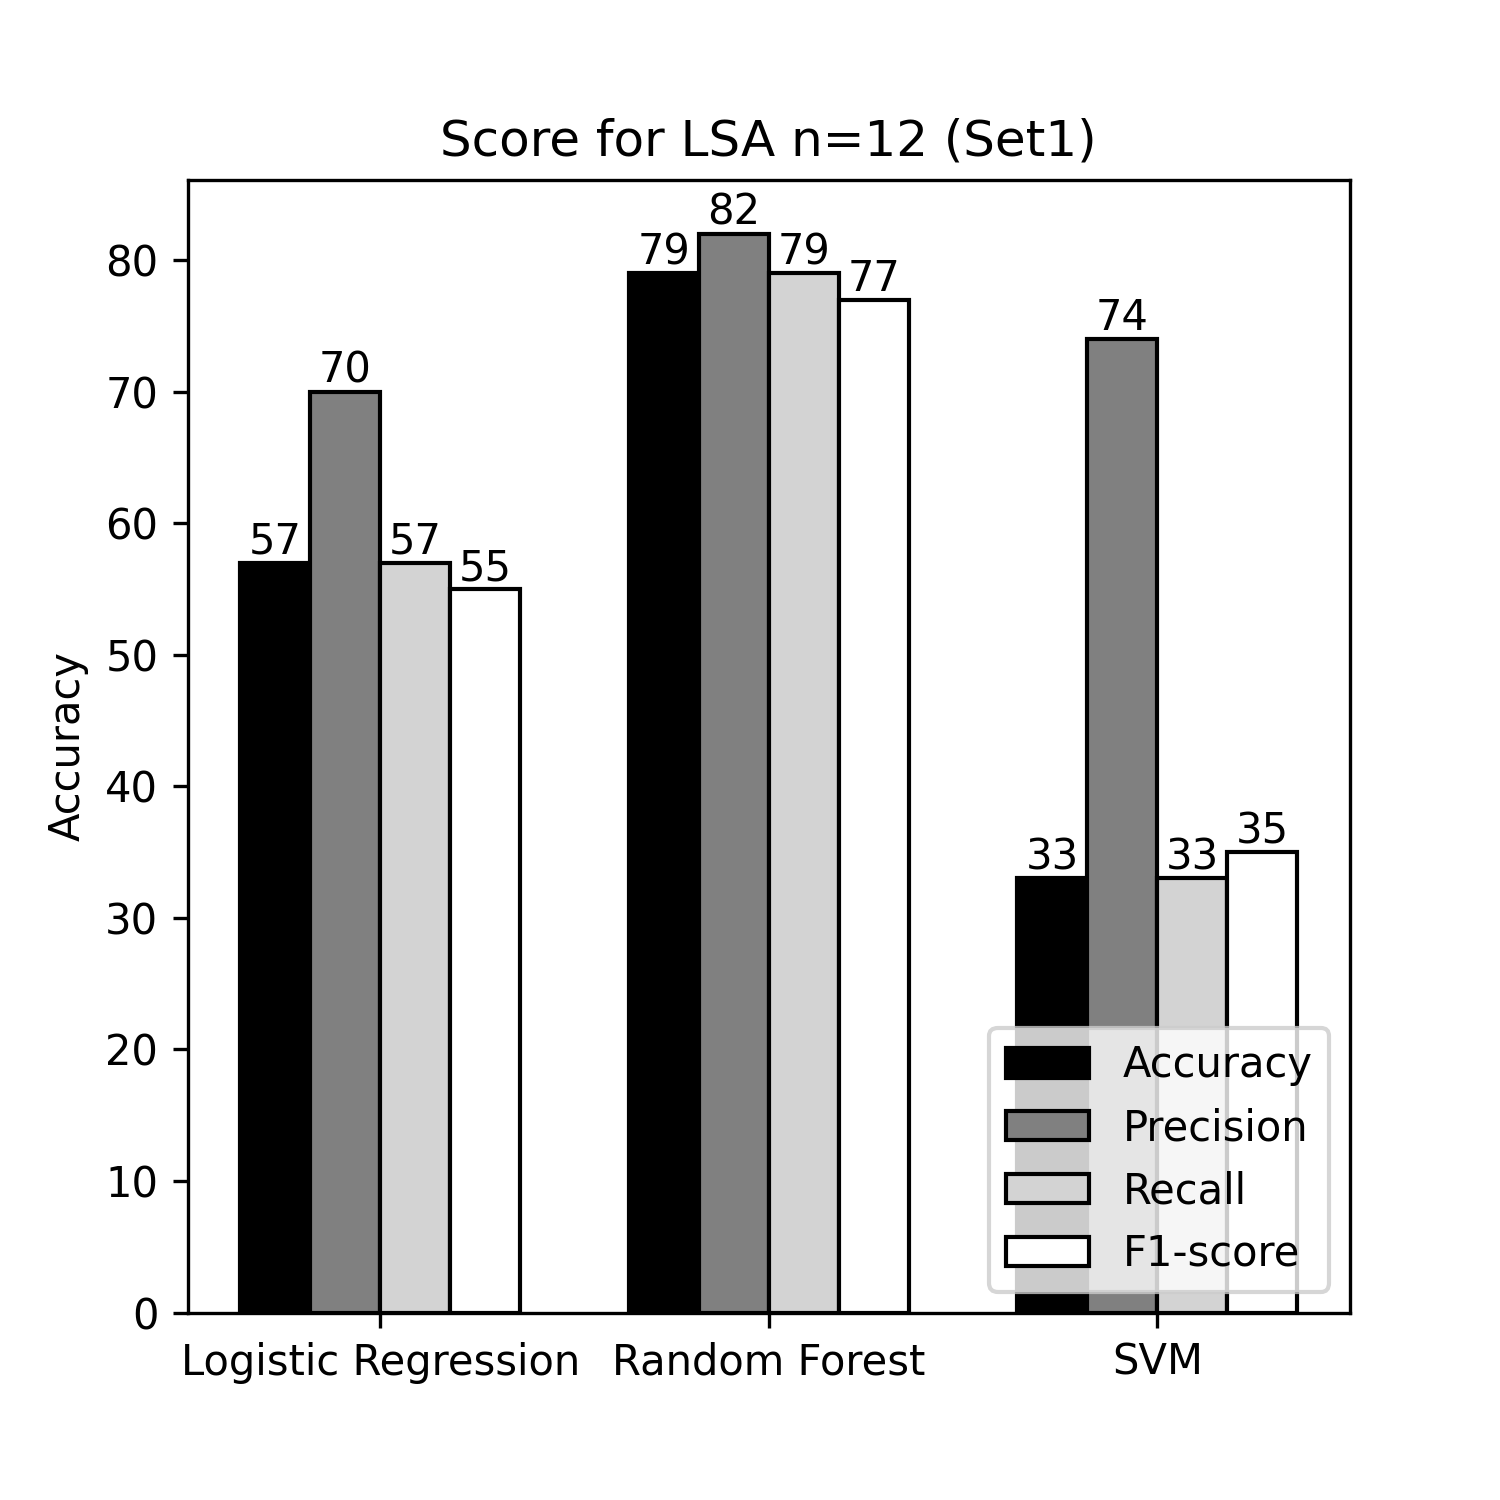
\includegraphics[scale=0.55]{plots/Score for LSA n=12 (Set1).png}
                  \caption{Score for LSA n=12 (Set1)}\label{Fig:typo2}
                \end{minipage}
             \end{figure}

             \begin{figure}[!htb]
                \begin{minipage}{0.48\textwidth}
                  \centering
                  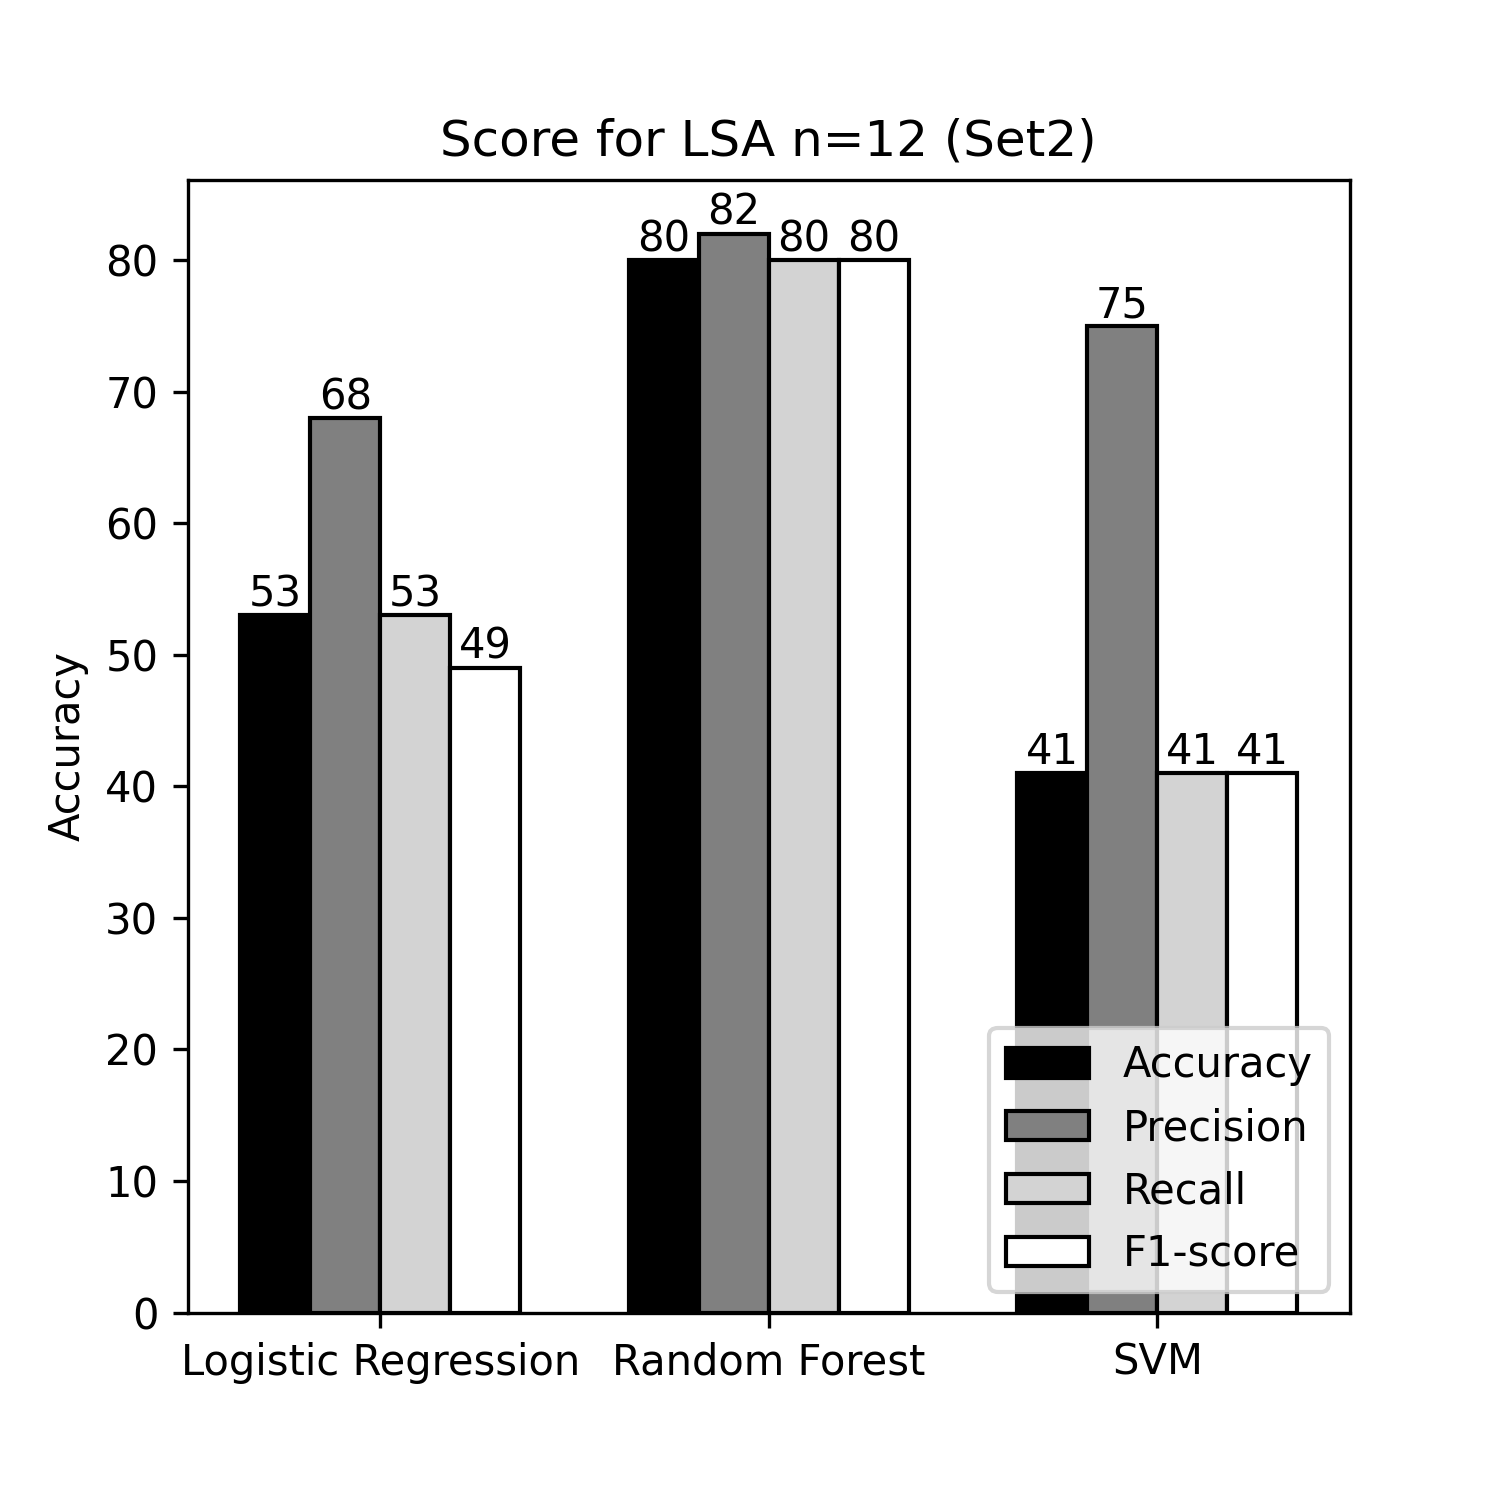
\includegraphics[scale=0.55]{plots/Score for LSA n=12 (Set2).png}
                  \caption{Score for LSA n=12 (Set2)}\label{Fig:typo1}
                \end{minipage}\hfill
                \begin{minipage}{0.48\textwidth}
                  \centering
                  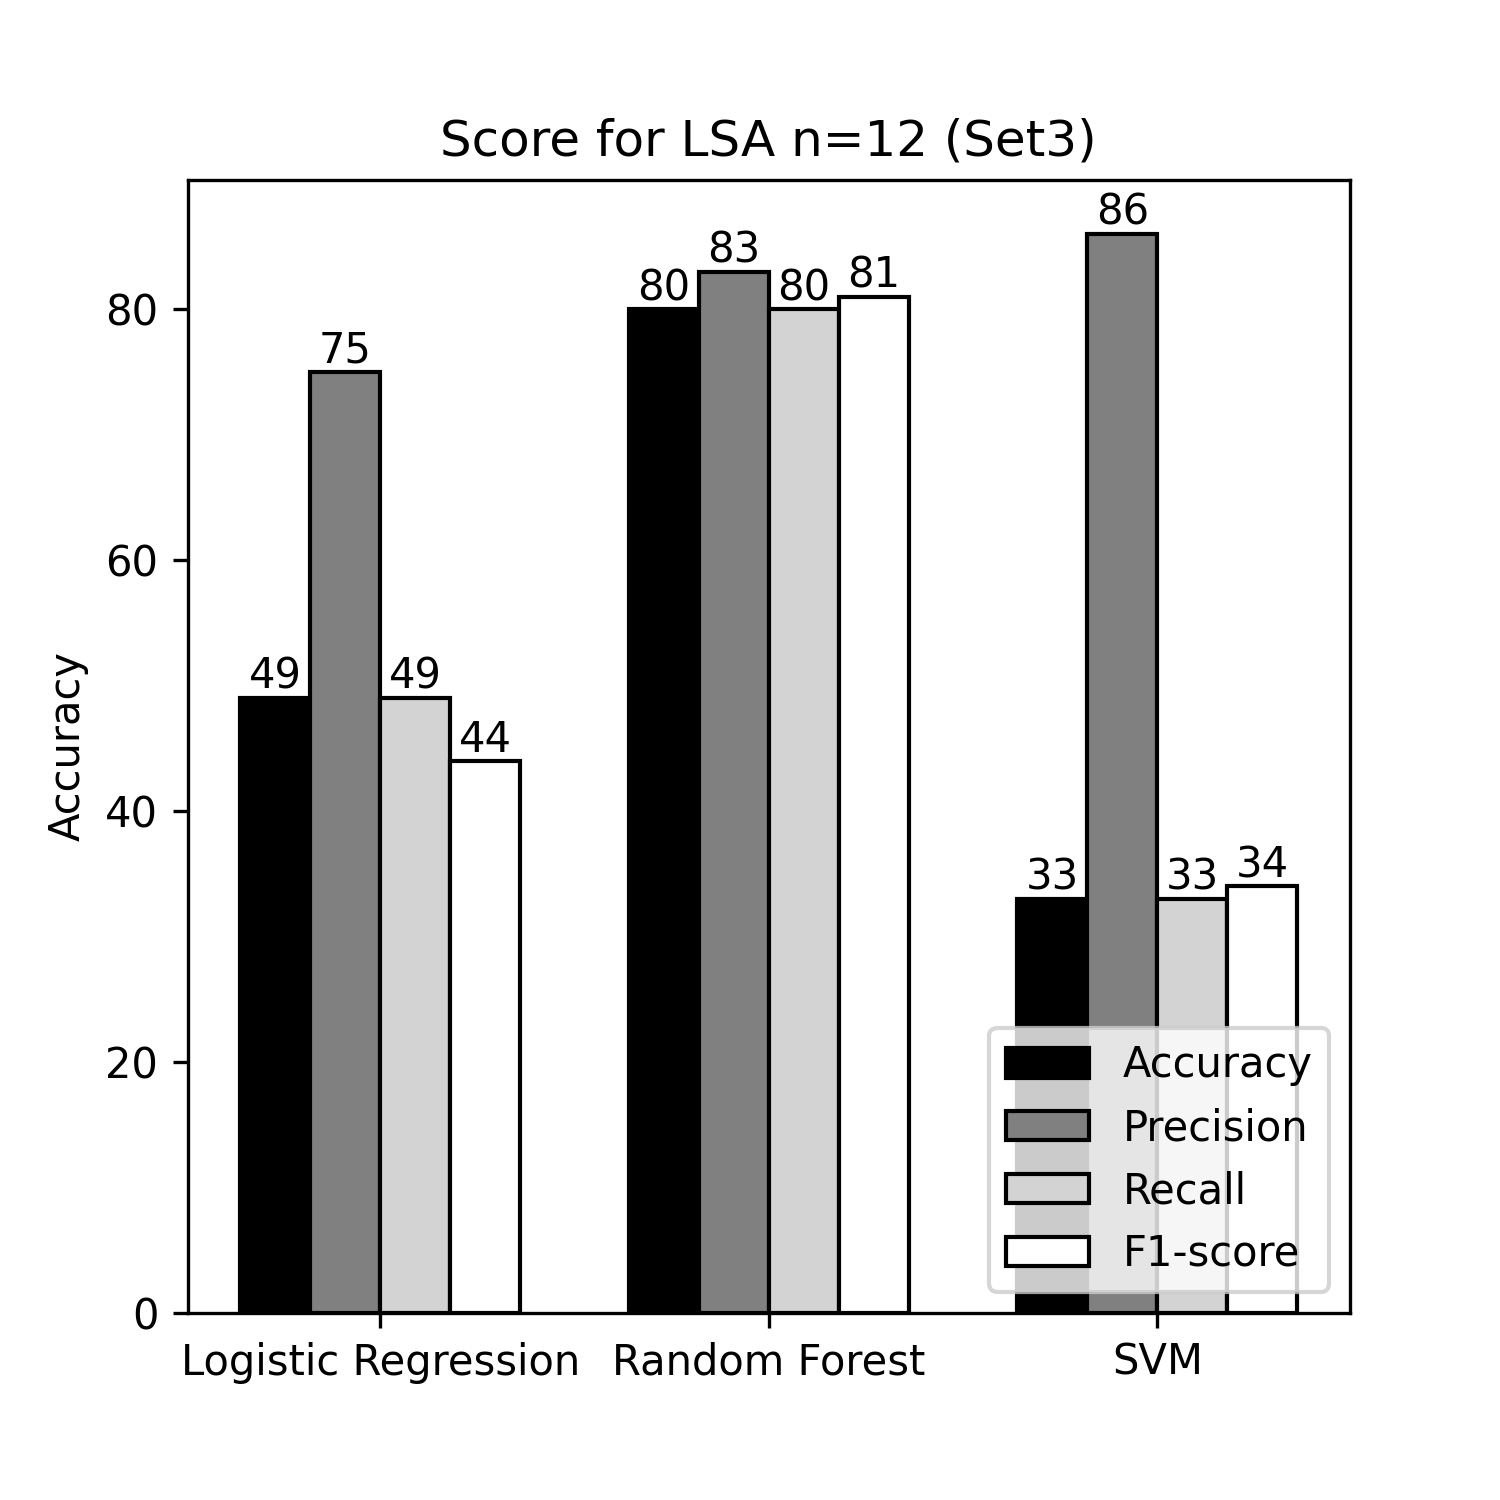
\includegraphics[scale=0.55]{plots/Score for LSA n=12 (Set3).png}
                  \caption{Score for LSA n=12 (Set3)}\label{Fig:typo2}
                \end{minipage}
             \end{figure}
 
            12 is clearly not suitable choice for feature extraction as shown in the figure 5.16 to 5.19. Almost all scores drop down to the bottom except random forest which 
            showed robustness in different scenarios. 


             \begin{figure}[!htb]
                \begin{minipage}{0.48\textwidth}
                  \centering
                  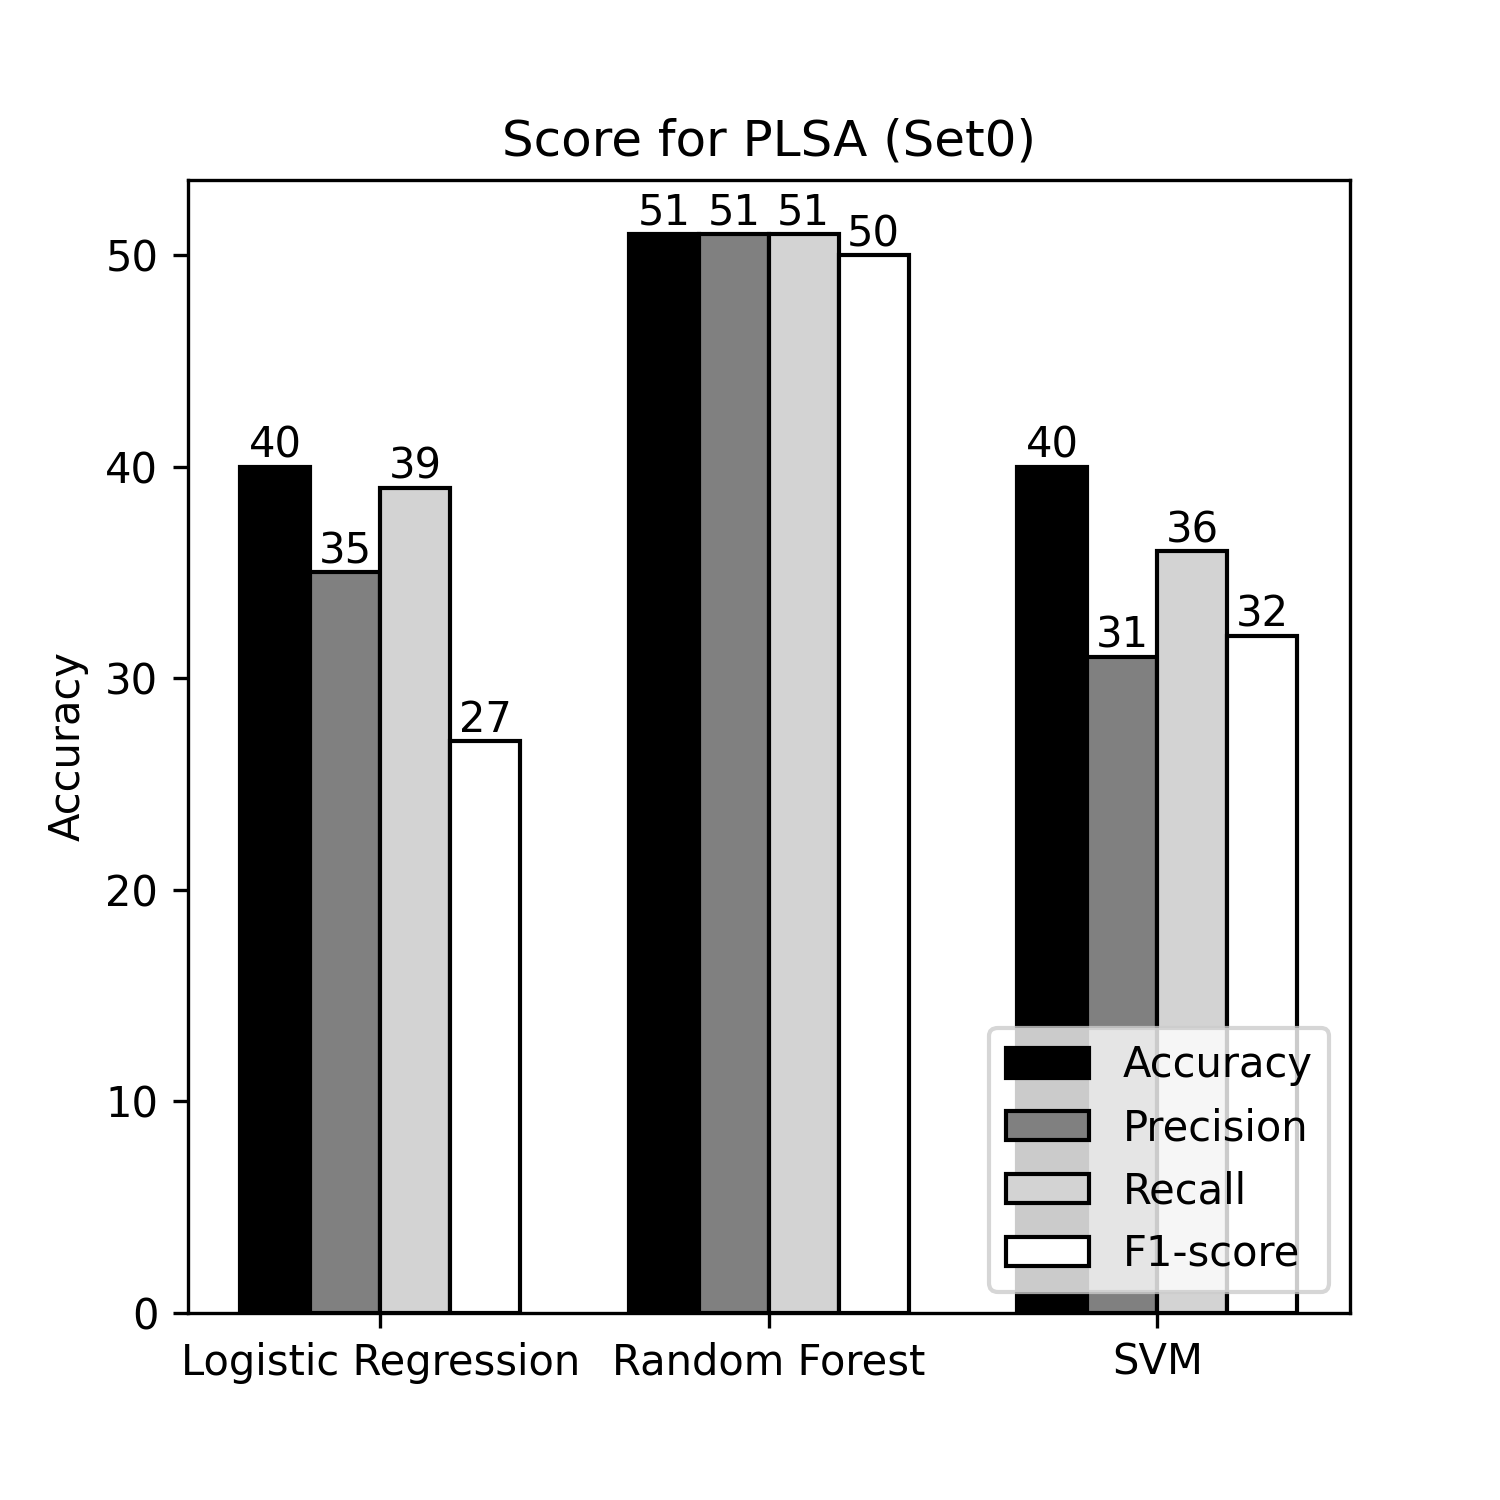
\includegraphics[scale=0.55]{plots/Score for PLSA (Set0).png}
                  \caption{Score for PLSA (Set0)}\label{Fig:typo1}
                \end{minipage}\hfill
                \begin{minipage}{0.48\textwidth}
                  \centering
                  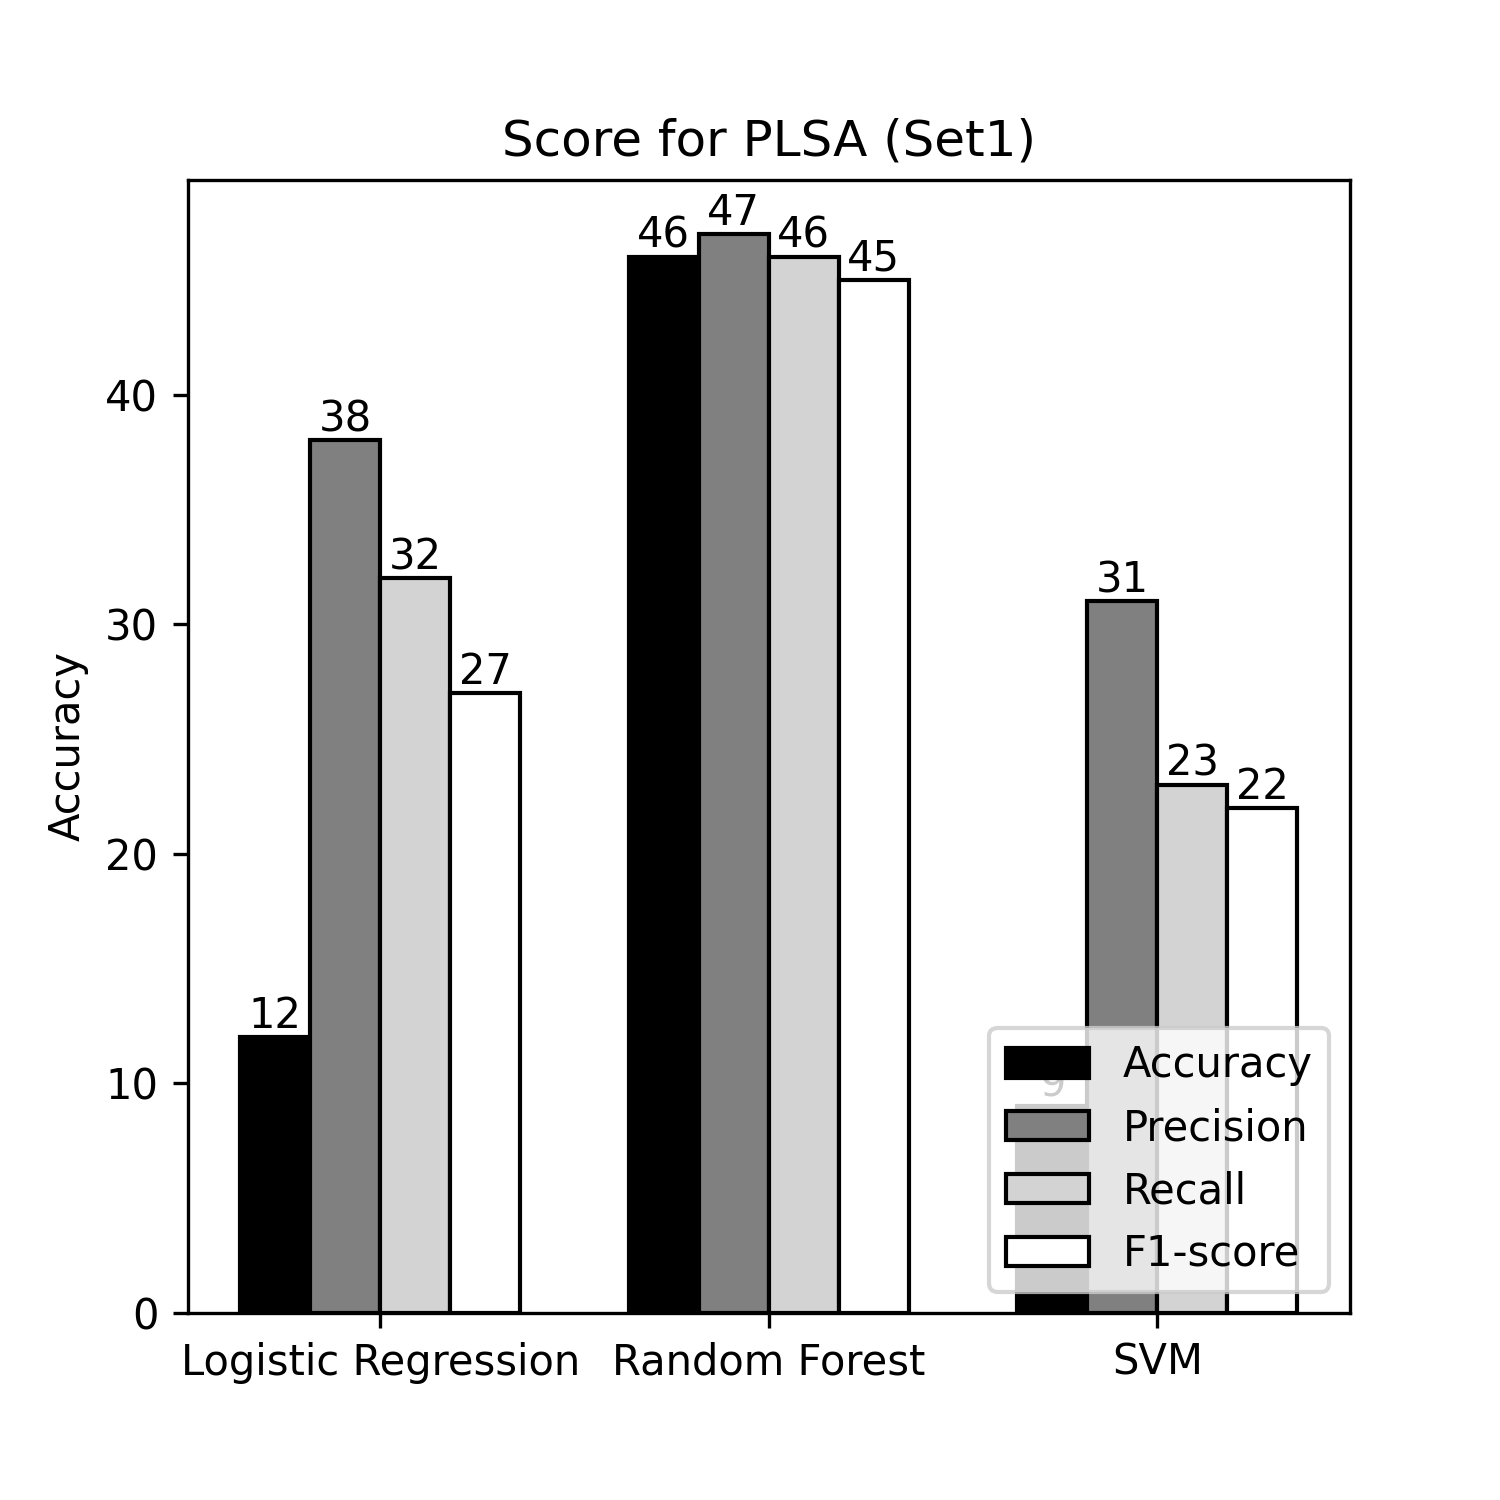
\includegraphics[scale=0.55]{plots/Score for PLSA (Set1).png}
                  \caption{Score for PLSA (Set1)}\label{Fig:typo2}
                \end{minipage}
             \end{figure}
            
             \begin{figure}[!htb]
                \begin{minipage}{0.48\textwidth}
                  \centering
                  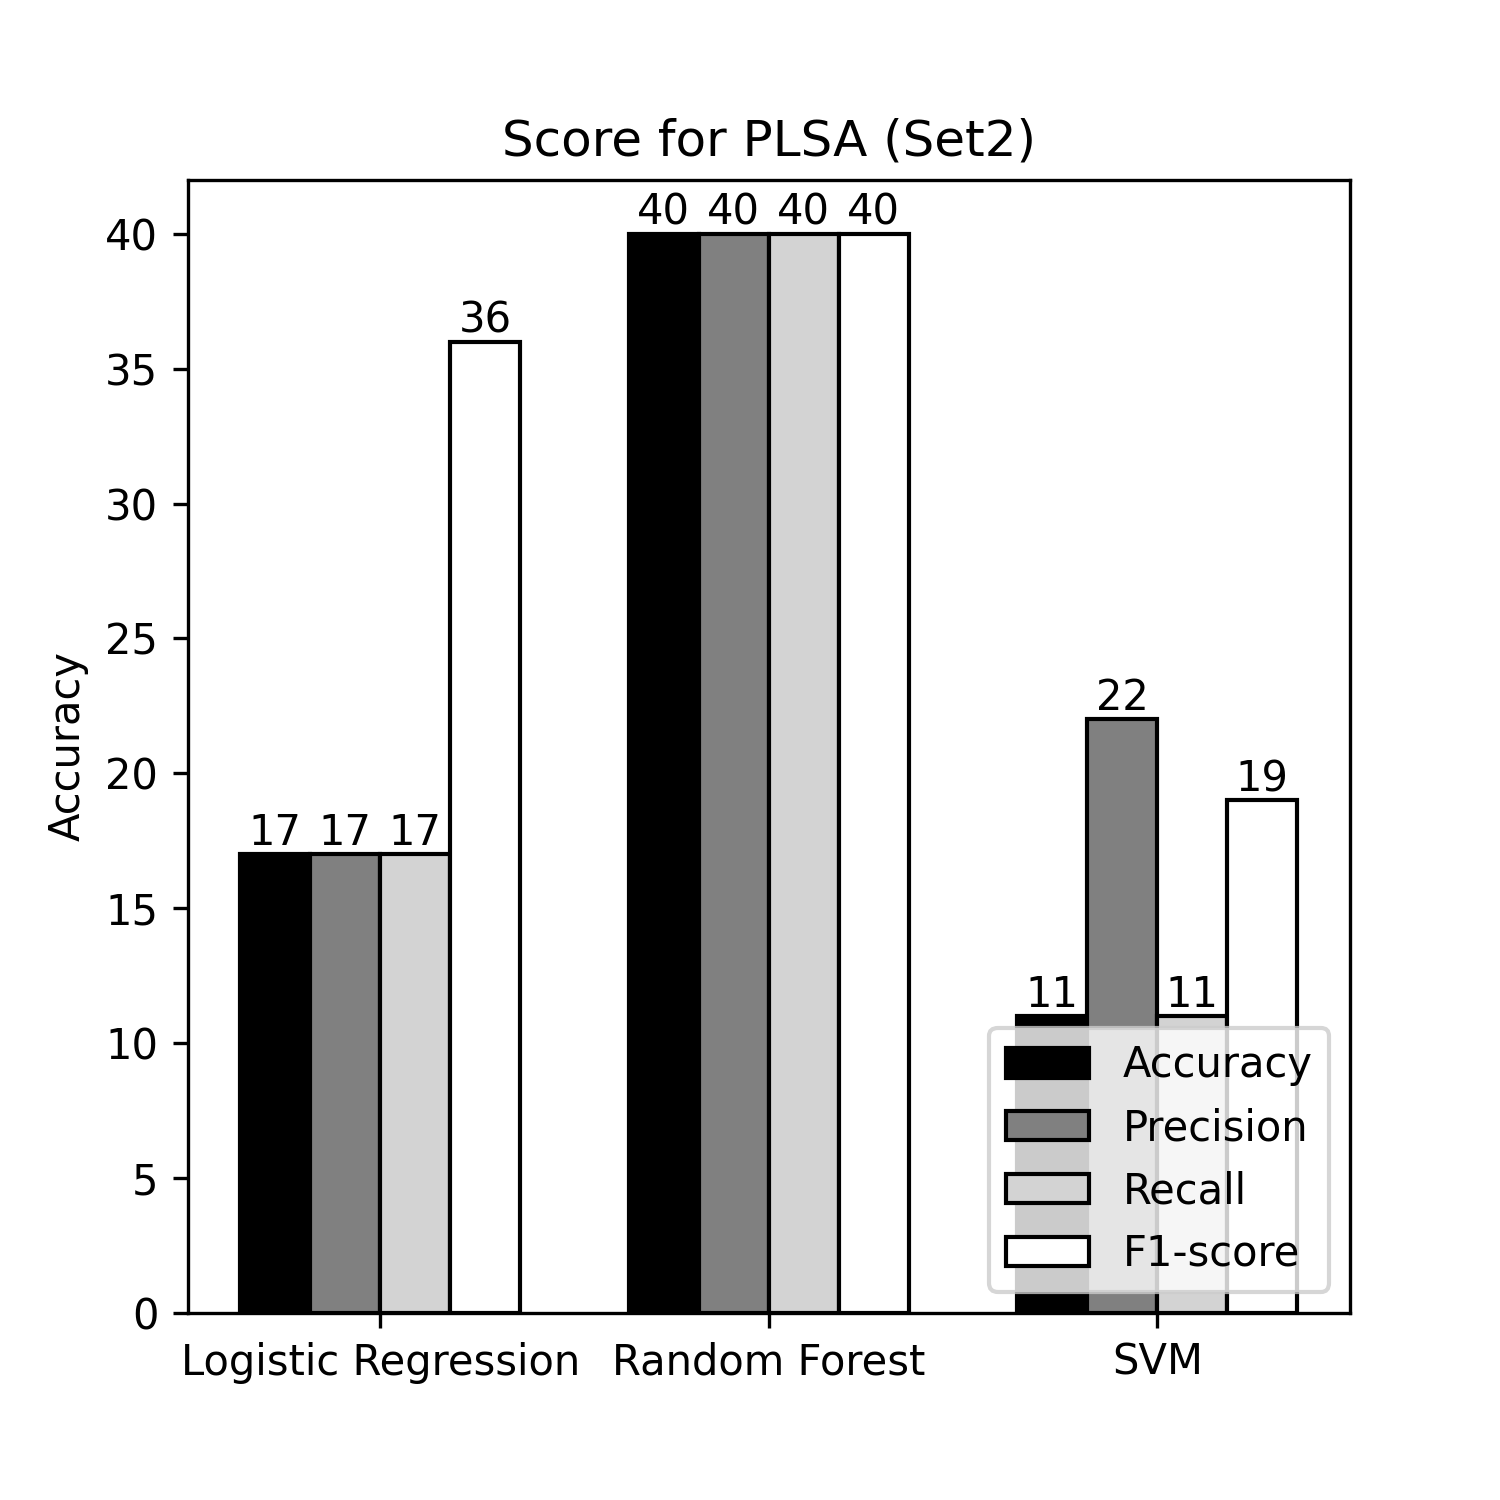
\includegraphics[scale=0.55]{plots/Score for PLSA (Set2).png}
                  \caption{Score for PLSA (Set1)}\label{Fig:typo1}
                \end{minipage}\hfill
                \begin{minipage}{0.48\textwidth}
                  \centering
                  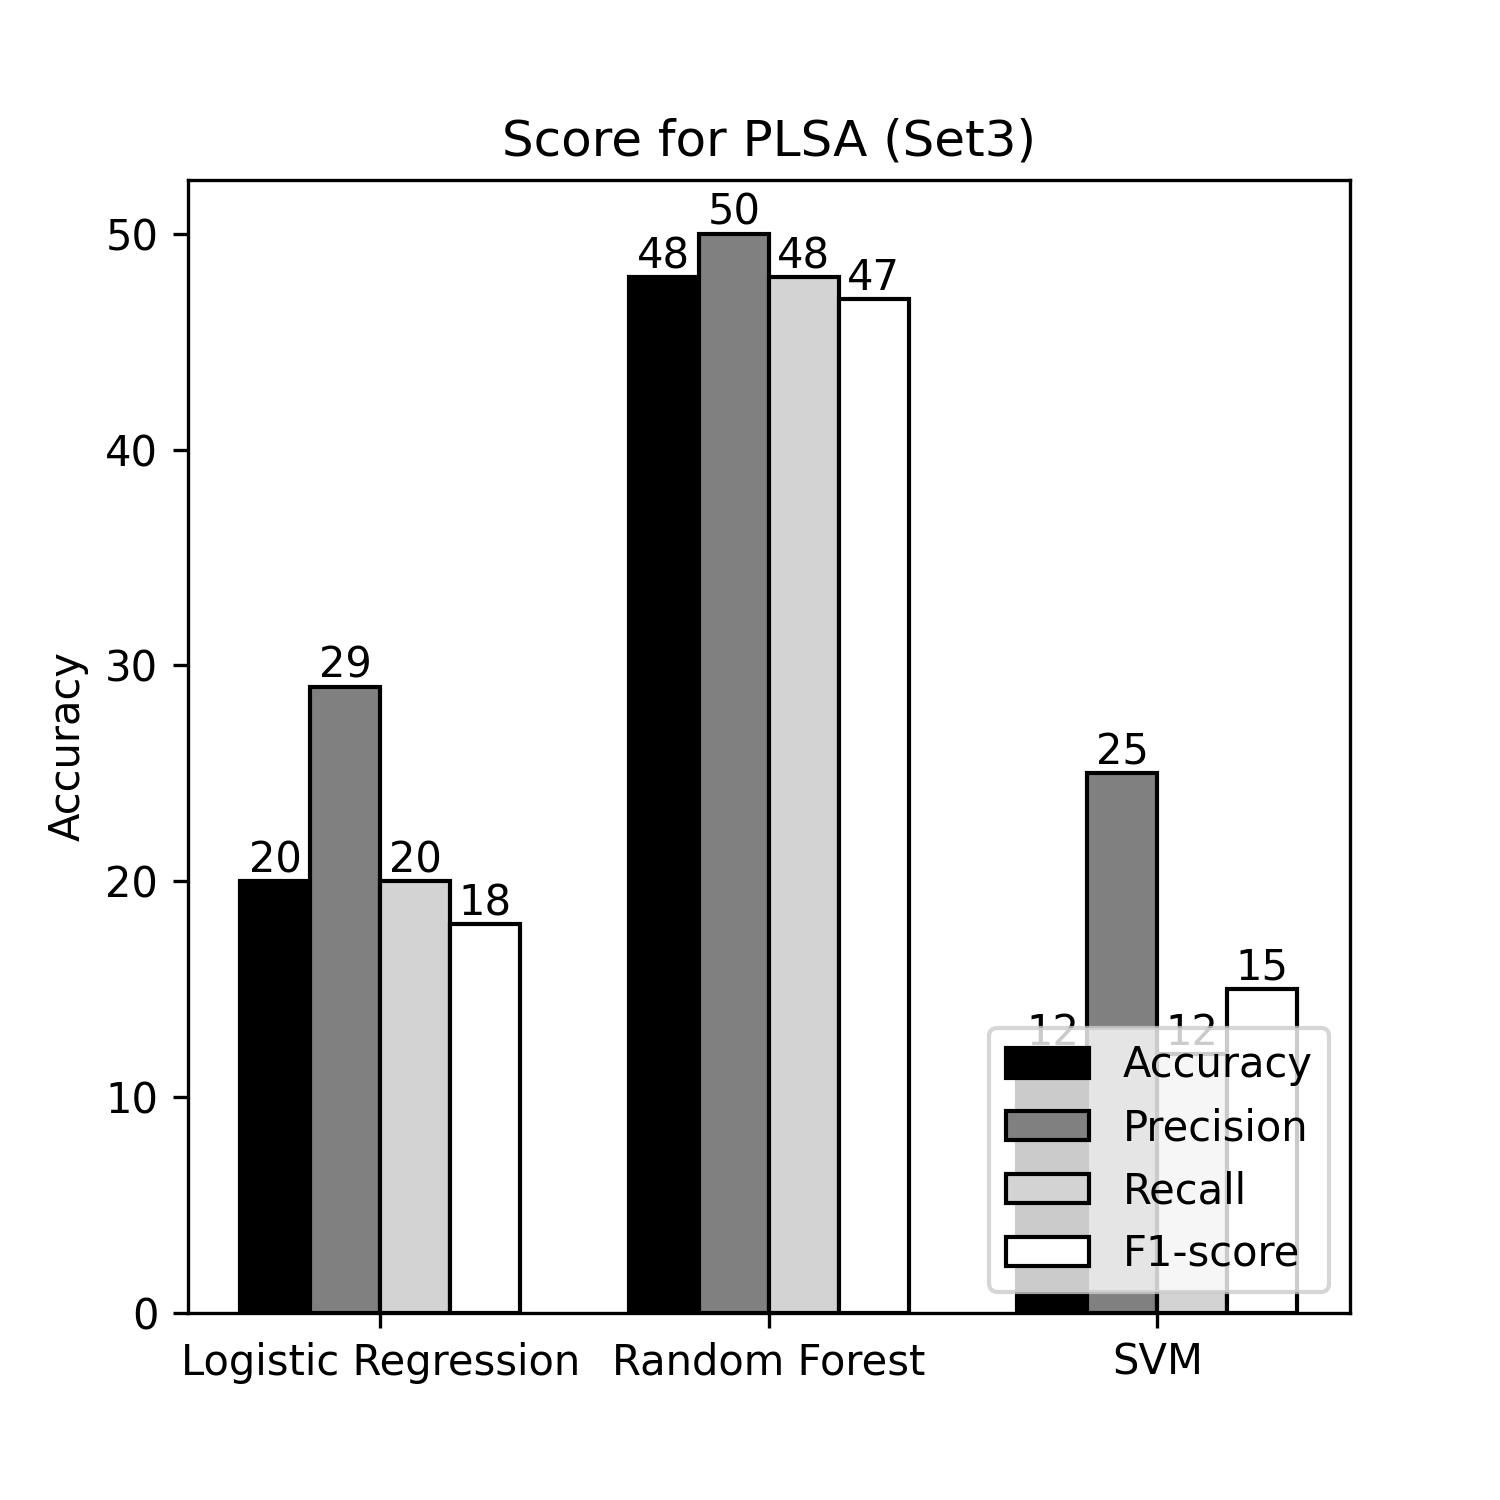
\includegraphics[scale=0.55]{plots/Score for PLSA (Set3).png}
                  \caption{Score for PLSA (Set3)}\label{Fig:typo2}
                \end{minipage}
             \end{figure}

             As PLSA is much more demanding in terms of computation operations and is much more time-consuming considering its iterative EM steps, calculating probability for each topic given document and word
             is rigorous on both memory and time complexity. So, PLSA performed worse compared to LSA for all machine learning algorithms, as the number of EM steps was not sufficient to maximize the expectation of the probablity for feature extraction. 
             Also, the constraints on resources, more data could not be processed to utilize the full potential of PLSA. In most datasets, evaluation scores were not upto par with LSA.  
             Even with the ensemble techinque, accuracy did not improve further than 50\%. 



             \chapter{Conclusion and Future Recommendations}
             \section{Conclusion}
             Hence, we found out that LSA performed significantly better than PLSA as feature extraction techinque. This might have been because of the lack of resource that we had to face
             during this project. 
             We also found that preprocessing techinques that are available to us today has a lot of room for improvement. Tools like stemmer and lemmatizer could 
             persuade the conclusions of projects such as ours to a different extent. Despite the limited amount of data and tools available for training the model. 
             
             The ensemble techinque seems to most benefit of this feature extraction techinque. Instead of manually extracting the features from the huge amount of unstructured 
             documents, we can use PLSA and LSA to increase efficieny in classification. These kinds of algorithms can be utilized for Nepali texts 
             and make better performing machine learning models.

             \section{Future Recommendations}

             Despite being a relatively simple algorithms, a lot of improvements can be made to further increase the performance of the feature extraction.
             Things like multi processing plsa can be made to make the algorithm run faster and more memory efficient. 
             We can also use the ratio of the sum of tf-idf of a given word to curate the data and filter out the unneeded features that are less significant 
             in the learning process of the model. 

             Also, using neural networks could make the process of feature extraction more easier and automatic. Although they also suffer from the need of 
             large amount of resources, they are significantly more powerful than simple machine learning algorithms.


                  


        % \section{Workflow of the Proposed System}
        % \begin{figure}[h]
        %     \centering
        %     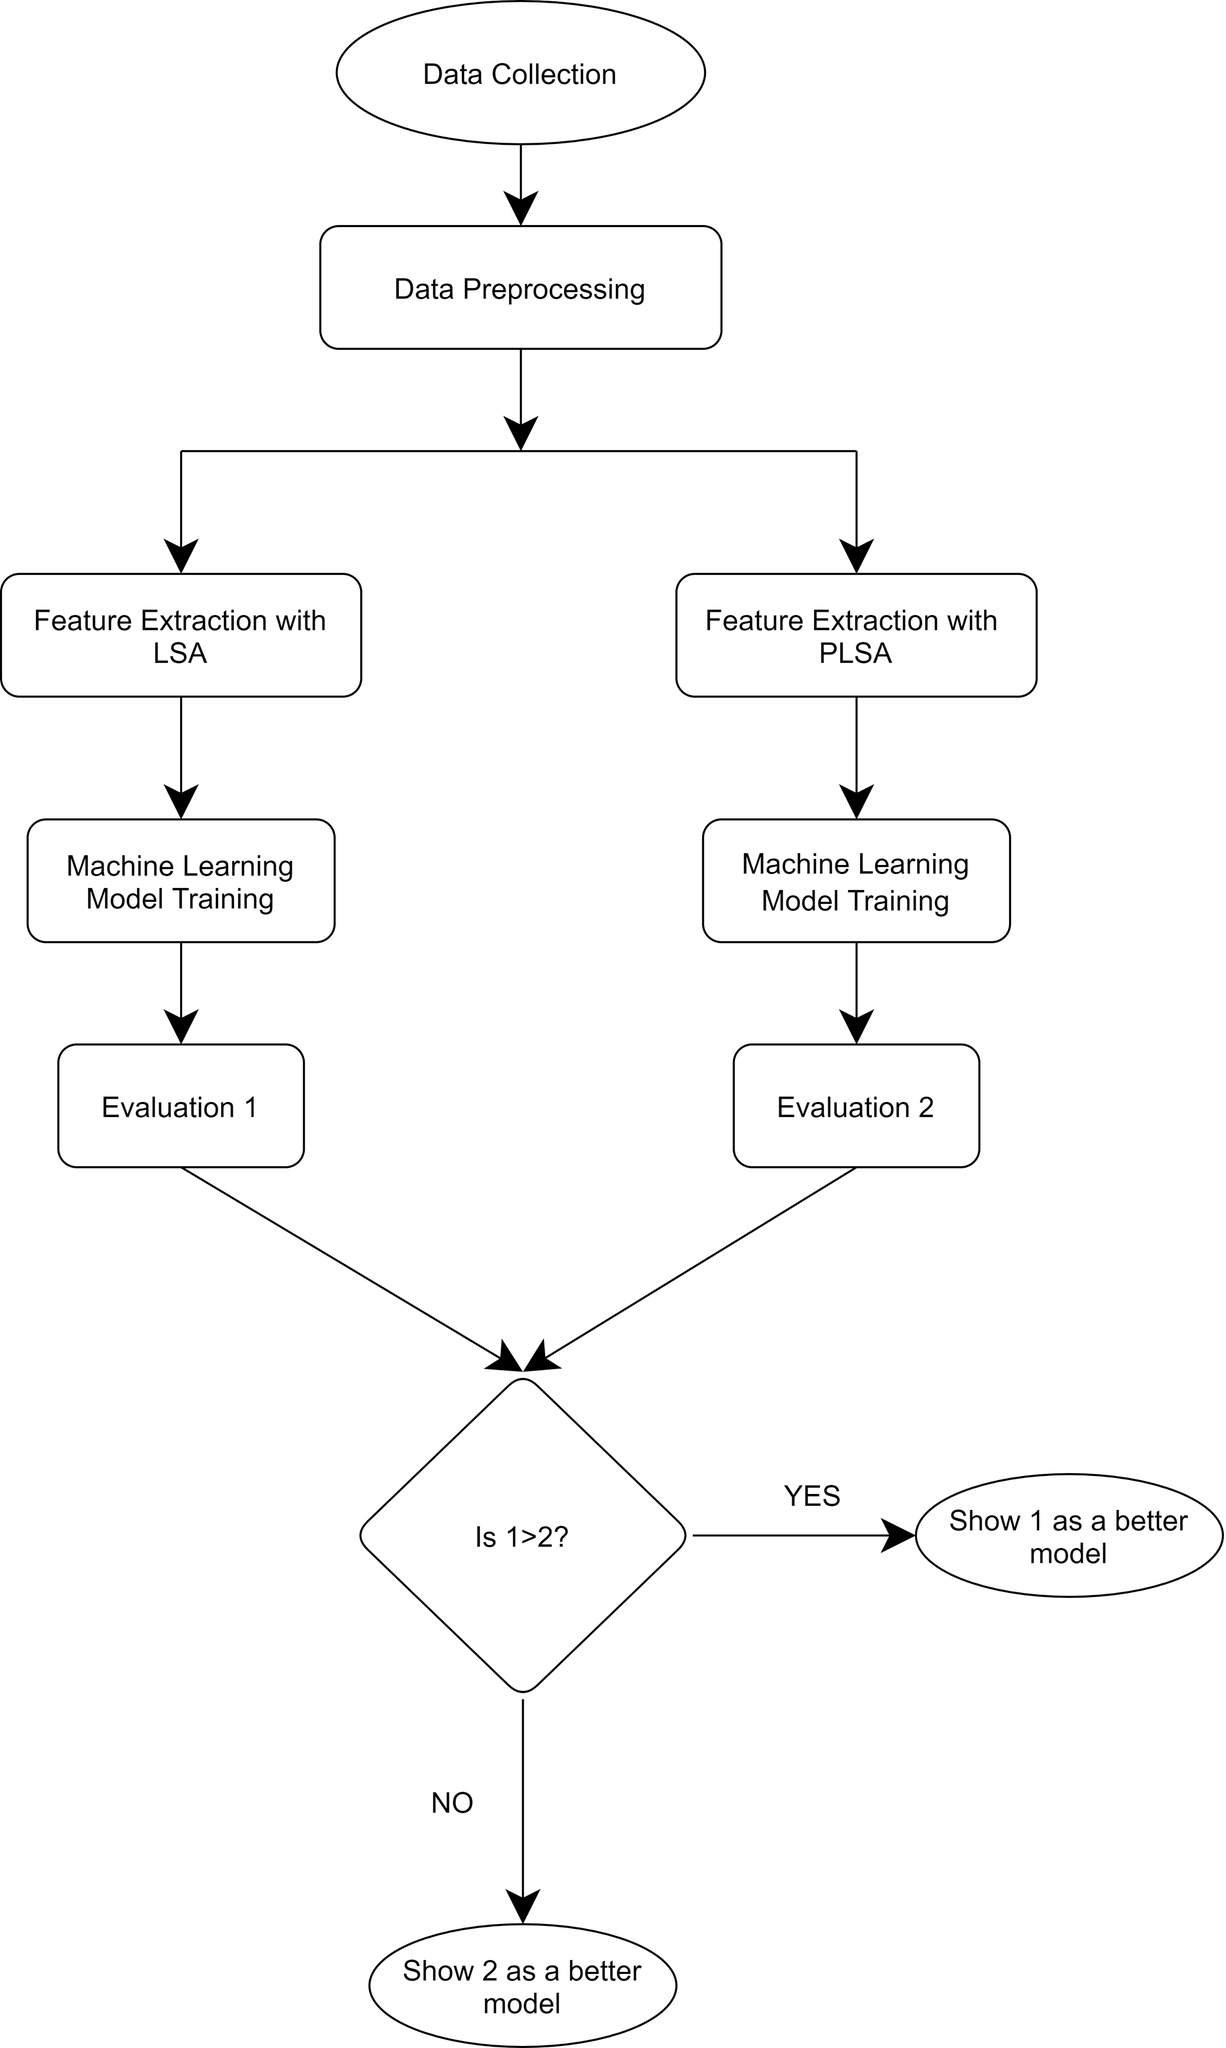
\includegraphics[width=12.29cm, height=18.25cm]{flowchart1.png}
        %     \caption{\textbf{The way the proposed system should operate.}}
        % \end{figure}

        

        % \section{Expected Outcome}
        % The system is expected to produce an outcome where one feature extraction technique is better than the other based on the different evaluation techniques. 

    \bibliography{references}
    \bibliographystyle{ieeetr}
\end{document}


